\documentclass[11pt,english]{article}
\usepackage[T1]{fontenc}
\usepackage[latin9]{inputenc}
\usepackage{geometry}
\geometry{verbose,tmargin=2cm,bmargin=2cm,lmargin=2cm,rmargin=2cm}
\setlength{\parskip}{\bigskipamount}
\setlength{\parindent}{0pt}
\usepackage{babel}
\usepackage{color}
\usepackage[capposition=top]{floatrow}
\usepackage{placeins}
\usepackage{subcaption}
\usepackage{array}
\usepackage{multirow}
\usepackage{amsmath}
\usepackage{amssymb}
\usepackage{graphicx}
\usepackage{afterpage}
%\usepackage{epstopdf}
\usepackage[outdir=./]{epstopdf} % Specify the output directory for pdf figures that are converted from eps. Without this, latex cannot read eps figures on mac.
%\usepackage{epstopdf}
%\epstopdfsetup{outdir=../figures/}
\usepackage{esint}
\usepackage[authoryear]{natbib}
\usepackage[unicode=true,pdfusetitle,
bookmarks=true,bookmarksnumbered=false,bookmarksopen=false,
breaklinks=false,pdfborder={0 0 1},backref=false,colorlinks=false]
{hyperref}
\hypersetup{
	citecolor=red,urlcolor=red,linkcolor=red}
\setcounter{MaxMatrixCols}{10}

\setcounter{MaxMatrixCols}{10}

\geometry{verbose}
\PassOptionsToPackage{normalem}{ulem}
\hypersetup{
	plainpages=false,urlcolor=magenta,citecolor=magenta,linkcolor=blue,pdfstartview=FitH,pdfview=FitH,plainpages=false,urlcolor=blue,citecolor=blue,linkcolor=blue,pdfstartview=FitH,pdfview=FitH}



\makeatletter

%%%%%%%%%%%%%%%%%%%%%%%%%%%%%% LyX specific LaTeX commands.
%% Because html converters don't know tabularnewline
\providecommand{\tabularnewline}{\\}

%%%%%%%%%%%%%%%%%%%%%%%%%%%%%% User specified LaTeX commands.


\newcommand*{\TabDir}{../tables}
\newcommand*{\FigDirSS}{../figures/ss}
\newcommand*{\FigDirG}{../figures/grant}  % transition with grant
\newcommand*{\FigDirNG}{../figures/nogrant} % transition without grant
\newcommand*{\FigDirGNG}{../figures/grant_vs_nogrant} % transition, comparison grant vs no grant

\def\indep{\perp\!\!\!\perp}


\def\limfunc#1{\mbox{\rm #1}\,}
\def\d{\,\mathrm{d}}

\usepackage{fullpage}
\usepackage{amsfonts}
\usepackage[titletoc]{appendix}
\usepackage[font=small,labelfont=bf]{caption}

\makeatother

\begin{document}

\title{Replication: Rescue Policies for small business during the COVID-19 recession, accepted for publication in the Review of Economic Dynamics}
\author{Alessandro Di Nola \and Leo Kaas \and Haomin Wang}
\date{\today}
\maketitle

\section{Steady-state}
\subsection{Calibration}
	
\begin{table}[htbp]
	\caption{\label{tab:nerd}Computational Parameters}
	\centering
	 \begin{tabular}{llc} \hline 
 Parameter & Description & Value \\ 
 \hline 
nx  & Num. of grid points for $x$       & 60 \\ 
nb  & Num. of grid points for $b$       & 80 \\ 
nk  & Num. of grid points for $\kappa$  & 100 \\ 
T   & Length of transition              & 180 \\ 
\hline 
 \end{tabular} 

\end{table}

\begin{table}[htbp]
	\caption{\label{tab:calib_external}External Parameters}
	
	\centering{}%
	 \begin{tabular}{llc} \hline 
 Parameter & Description & Value \\ 
 \hline 
$\beta$  & Subjective discount factor &    0.989 \\ 
$\sigma$  & CRRA coefficient &    2.000 \\ 
$\alpha$  & Capital Share corporate sector &    0.300 \\ 
$\delta_k$  & Capital depreciation rate &    0.015 \\ 
$\lambda_0$  & Collateral constraint parameter &    1.000 \\ 
$\gamma_1$  & Capital Share small firms &    0.318 \\ 
$\gamma_2$  & Span of control &    0.880 \\ 
$A$  & TFP shifter &    0.250 \\ 
$bk0(1)$  & Initial debt-asset ratio &   -0.094 \\ 
$bk0(2)$  & Initial debt-asset ratio &    0.125 \\ 
$bk0(3)$  & Initial debt-asset ratio &    0.868 \\ 
$Pr(bk0(1))$  & Prob. dist. &    0.250 \\ 
$Pr(bk0(2))$  & Prob. dist. &    0.500 \\ 
$Pr(bk0(3))$  & Prob. dist. &    0.250 \\ 
\hline 
 \end{tabular} 

\end{table}

\begin{table}[htbp]
	\caption{Estimated Parameter Values}
   	\label{tab:parameters}\centering
   	 \begin{tabular}{llc} \hline \hline 
 Parameter & Description & Value \\ 
 \hline 
$ M $  & mass of potential entrants &    0.045 \\ 
$ fixcost1  $  & Intercept fixed cost &    0.165 \\ 
$ fixcost2  $  & Slope fixed cost &    0.005 \\ 
$ \theta $  & Resale value of capital &    0.909 \\ 
$ \psi $  & Exogenous exit rate &    0.004 \\ 
$ \alpha_{\kappa}  $  & Shape Pareto capital &    0.446 \\ 
$ \bar{x}    $  & Ln(x0) mean of AR(1) &    1.074 \\ 
$ \varepsilon_x    $  & Dispersion of $x$ &    0.098 \\ 
$ \rho_x    $  & Persistence of $x$ &    0.957 \\ 
$ \zeta    $  & marginal utility of leisure &   23.420 \\ 
\hline \hline 
 \end{tabular} 

\end{table}

\begin{table}[htbp]
	\caption{Steady state results}
	\label{tab:steady_state}\centering
	 \begin{tabular}{lc} \hline \hline 
 \hline 
Measure of active firms:   &    0.0171  \\ 
Measure of entrants:       &    0.0004  \\ 
Aggregate consumption:     &    0.1084  \\ 
Capital (corporate):       &    0.7526  \\ 
Employment (corporate):    &    0.1668  \\ 
Aggregate Capital:         &    1.2399  \\ 
Employment (total):        &    0.3175  \\ 
Output (corporate):        &    0.0655  \\ 
Output (small firms):      &    0.0639  \\ 
Total output:              &    0.1295  \\ 
liq:                       &    0.0019  \\ 
entry:                     &    0.0004  \\ 
Aggregate Investment:      &    0.0211  \\ 
btilde(1):                 &  -1062.0793  \\ 
btilde(nk):                &  -871.6766  \\ 
\hline \hline 
 \end{tabular} 

\end{table}


\begin{table}[htbp]
	\caption{Model Fit}
    \label{tab:moments}\centering
     \begin{tabular}{lcc} \hline \hline 
 Moment & Data & Model \\ 
\hline 
Average employment in small firms  &    9.2516 &   8.8026 \\ 
Average employment, age 0  &    5.2935 &   5.3071 \\ 
Small firm share of employment  &    0.4895 &   0.4746 \\ 
Small firm exit rate  &    0.0198 &   0.0210 \\ 
Fixed expense to revenue ratio  &    0.2448 &   0.2286 \\ 
Autocorr. employment  &    0.9667 &   0.9527 \\ 
Time spent in market work  &    0.3300 &   0.3175 \\ 
Exit rate, emp. size 0 to 9  &    0.0246 &   0.0251 \\ 
serial corr. investment rate  &    0.0580 &   0.0591 \\ 
Share of firms with debt  &    0.3288 &   0.2190 \\ 
Freq. positive lumpy investment  &    0.1860 &   0.2123 \\ 
Share forced exit  &    1.0000 &   0.5362 \\ 
Share voluntary exit  &    1.0000 &   0.3147 \\ 
firmshare0to9  &    0.7921 &   0.8052 \\ 
firmshare10to19  &    0.1039 &   0.0779 \\ 
firmshare20to99  &    0.0869 &   0.1061 \\ 
firmshare100to499  &    0.0171 &   0.0108 \\ 
empshare0to9  &    0.2286 &   0.1891 \\ 
empshare10to19  &    0.1499 &   0.1247 \\ 
empshare20to99  &    0.3510 &   0.5244 \\ 
empshare100to499  &    0.2705 &   0.1618 \\ 
\hline \hline 
 \end{tabular} 

\end{table}


\begin{figure}[htbp]
	\centering
	\begin{subfigure}[b]{0.46\textwidth}
		\centering
		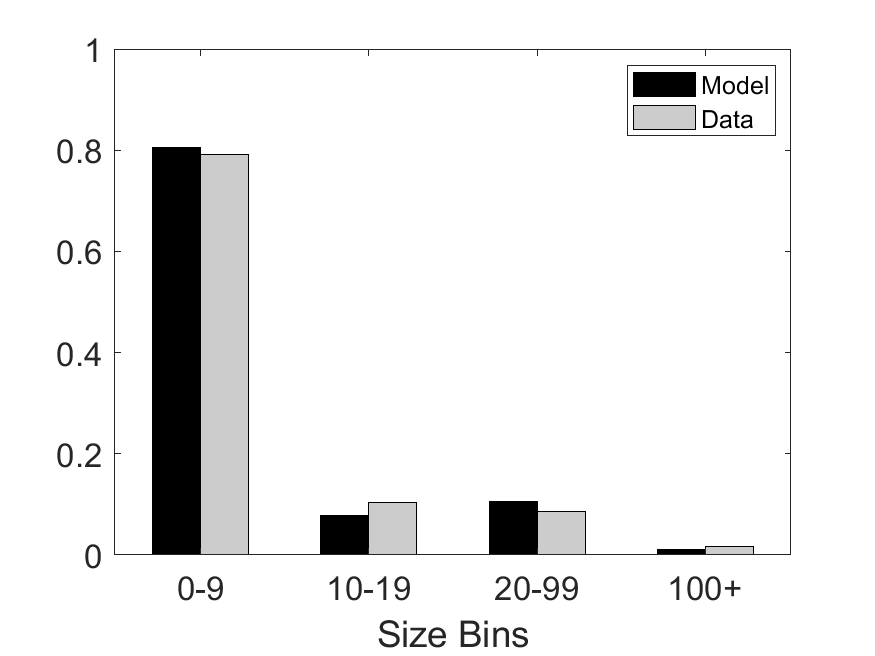
\includegraphics[width=\textwidth]{\FigDirSS/firmSize}
		\caption{Firm size distribution}
	\end{subfigure} \hfill
	\begin{subfigure}[b]{0.46\textwidth}
		\centering
		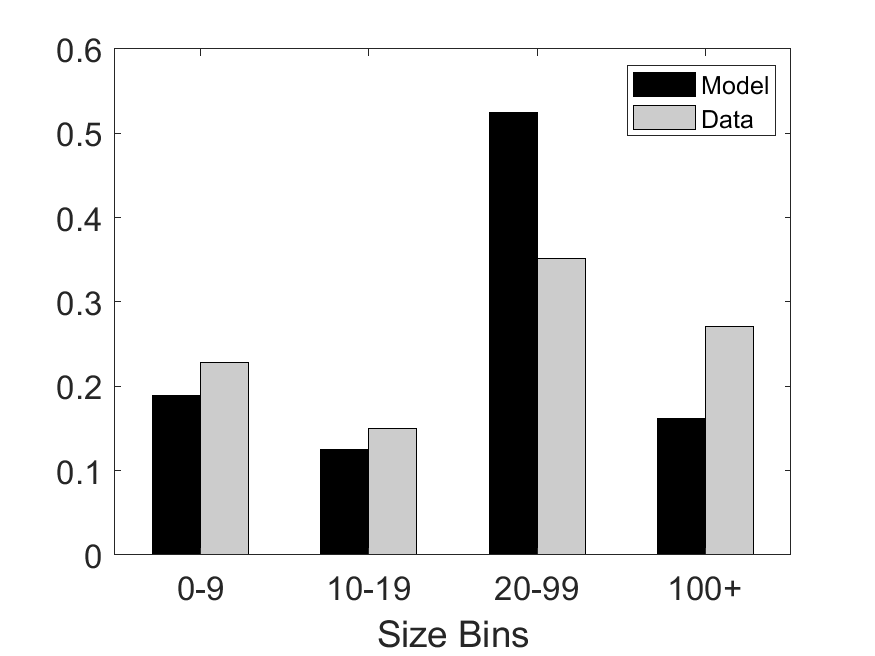
\includegraphics[width=\textwidth]{\FigDirSS/empShare}
		\caption{Employment distribution}
	\end{subfigure}
	\caption{Firm size and employment distributions: Model vs Data}
	\label{fig:bins}
\end{figure}
    
\FloatBarrier

\subsection{Steady state policy functions}

    \begin{figure}[htbp]
    	\centering
    		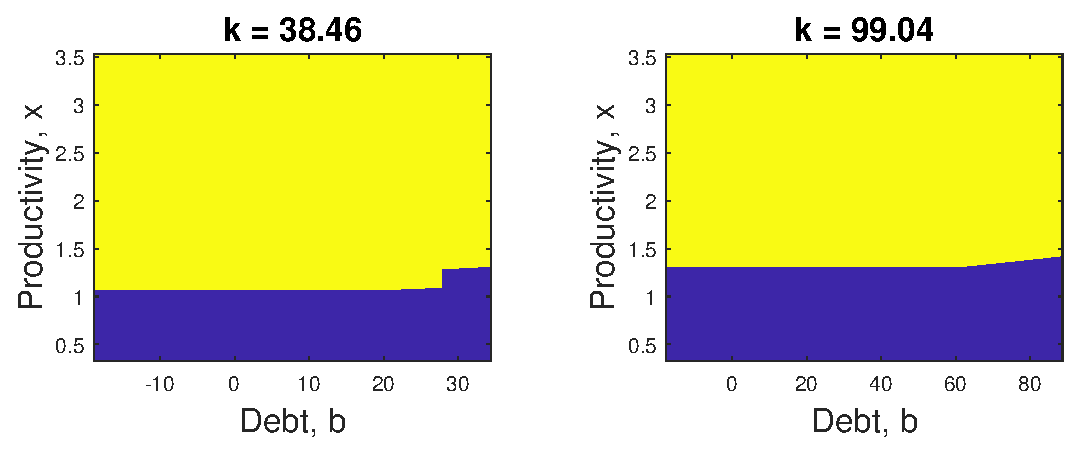
\includegraphics[width=0.7\textwidth]{\FigDirSS/entry_type_ss}
    		\caption{Entry policy}	
    		{\textit{Notes:} \raggedright Yellow = entry, blue = no entry.  \par}
    \end{figure}

	\begin{figure}[htbp]
	 	\centering
			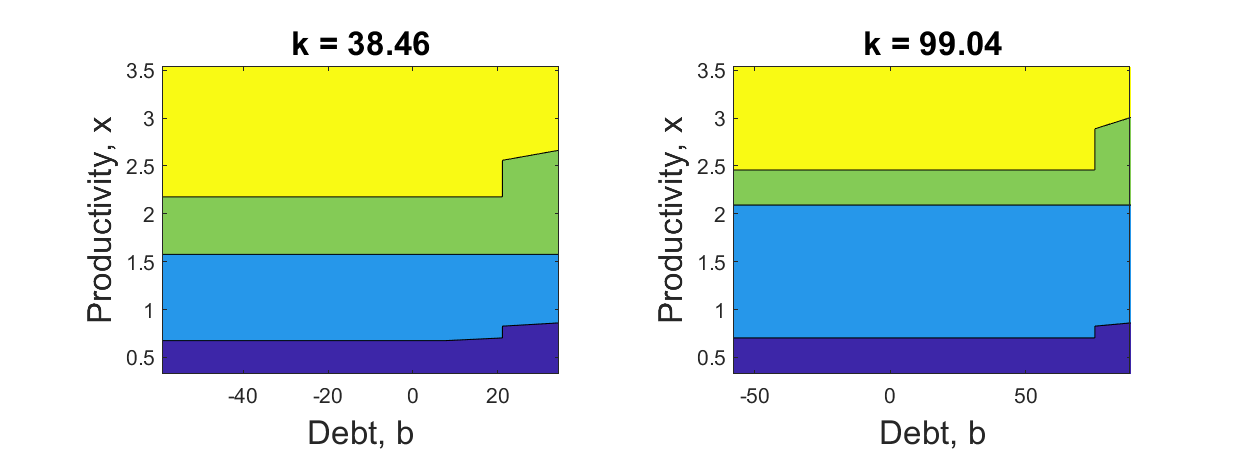
\includegraphics[width=\textwidth]{\FigDirSS/inv_type_ss}
			\caption{Investment type. Dark blue: exit, light blue: negative investment (no exit), Green: small positive investment (investment rate less than 100\%), yellow: large positive investment (investment rate greater than 100\%). }
	\end{figure}


\begin{figure}[htbp]
	\centering
		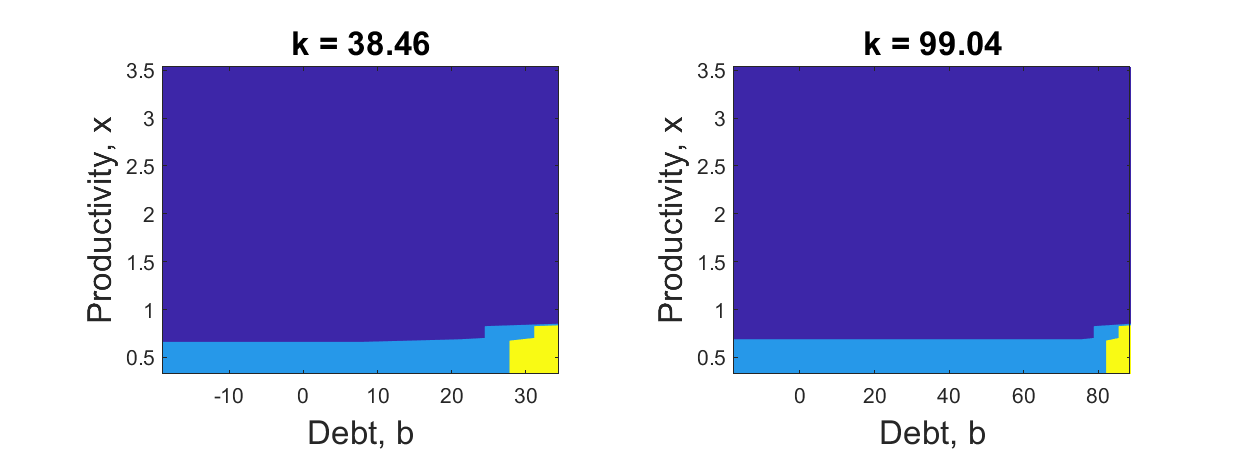
\includegraphics[width=\textwidth]{\FigDirSS/exit_type_ss}
		\caption{Exit type. Dark blue: no exit, yellow: forced exit, light blue: voluntary exit.}
\end{figure}

\FloatBarrier
	
\section{Transition \label{sec:irf}}
	
\subsection{Calibration of transition}

We assume that the pandemic impacts a fraction $\eta_i$ of small firms. Those impacted see their productivity $x$ goes to zero; the unimpacted firms' productivity is unaffected by the pandemic.

\begin{table}[htbp]
	 \begin{tabular}{llc} \hline 
 Parameter & Description & Value \\ 
 \hline 
$ \eta_{i}$ & Fraction of impacted small firms &   0.1200 \\ 
$ \nu^{n}$ & Productivity shock on impacted firms &  -1.0000 \\ 
$ \nu^{\lambda}$ & Credit shock on small firms &  -0.1580 \\ 
$ \nu^{M}$ & Shock to the mass of potential entrants &   0.2400 \\ 
$ \nu^{c}$ & Productivity shock the corporate sector &  -0.0070 \\ 
$ \nu^{d}$ & Preference shock                  &  -0.1843 \\ 
$ \nu^{l}$ & Labor supply shock                &   0.2500 \\ 
$ \rho   $ & Autocorrelation                   &   0.1100 \\ 
\hline 
 \end{tabular} 

	\caption{Calibrated Pandemic Shock Parameters}
\end{table}
	
\bigskip
	
\begin{table}[H]
	 \begin{tabular}{lcc} \hline \hline 
 Description & Data & Model      \\ 
 \hline 
Output, 2020Q2            & -10.8570 & -10.8976   \\ 
Output, 2020Q3            &  -2.2460 &  -2.4738   \\ 
Consumption, 2020Q2        &  -9.6670 &  -9.8018   \\ 
Total employment, 2020Q2     & -12.8500 & -11.7066   \\ 
Employment small, 2020Q2      & -16.0213 & -16.2132   \\ 
Exit rate, 2020Q2       &  37.8400 &  37.7459   \\ 
Entry rate, 2020Q2       & -12.5000 & -12.1711   \\ 
Private investment, 2020Q2         & -15.3980 & -16.5231   \\ 
Small firm output, 2020Q2 & -15.6500 & -15.8452   \\ 
\hline \hline 
 \end{tabular} 

	\caption{Pandemic Impact and Rescue Policies}
	\label{tab:transition}

	\vspace{1ex}
	{\textit{Notes:} \raggedright The pandemic shocks are calibrated so that the ``Grant baseline'' economy matches the data. \textit{Data sources:} GDP, consumption, investment and aggregate employment come from FRED. Small firms output comes from Bloom et al. (2021), Figure A7. Employment by firm size comes from ADP, see Cajner et al. (2020). Exit and entry rate comes from BED. \par}
\end{table}

      
\begin{figure}[htbp]
	\centering
	\begin{subfigure}[b]{0.45\textwidth}
		\centering
		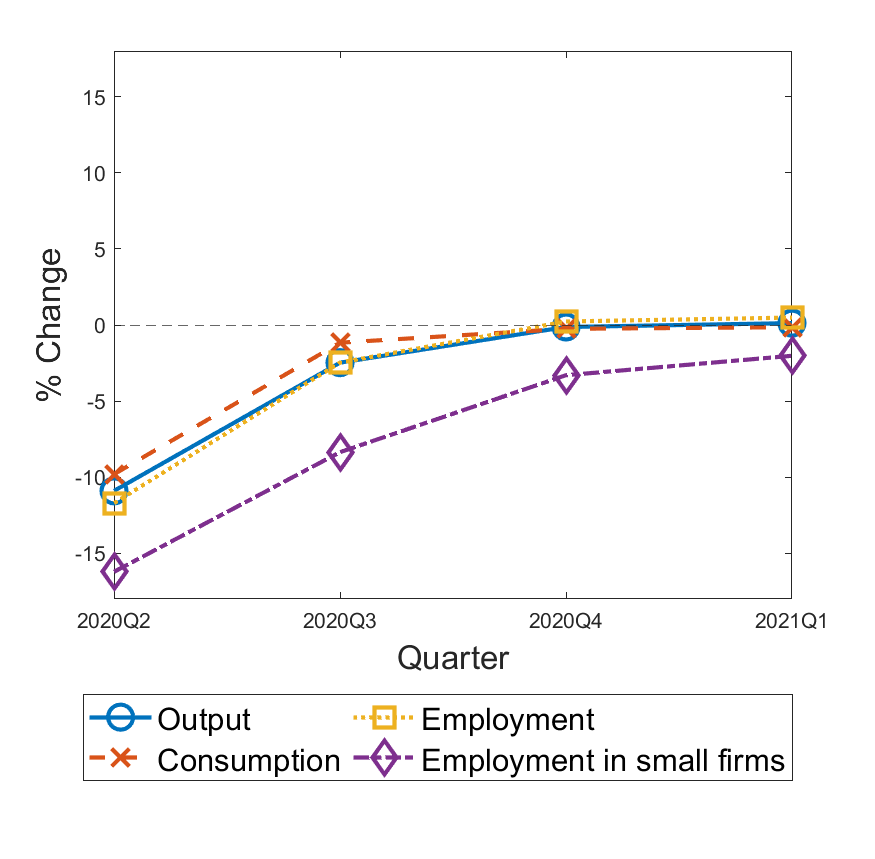
\includegraphics[width=\textwidth]{\FigDirGNG/model_mom_trans}
		\caption{Calibrated shocks}
	\end{subfigure} \hfill
	\begin{subfigure}[b]{0.45\textwidth}
		\centering
		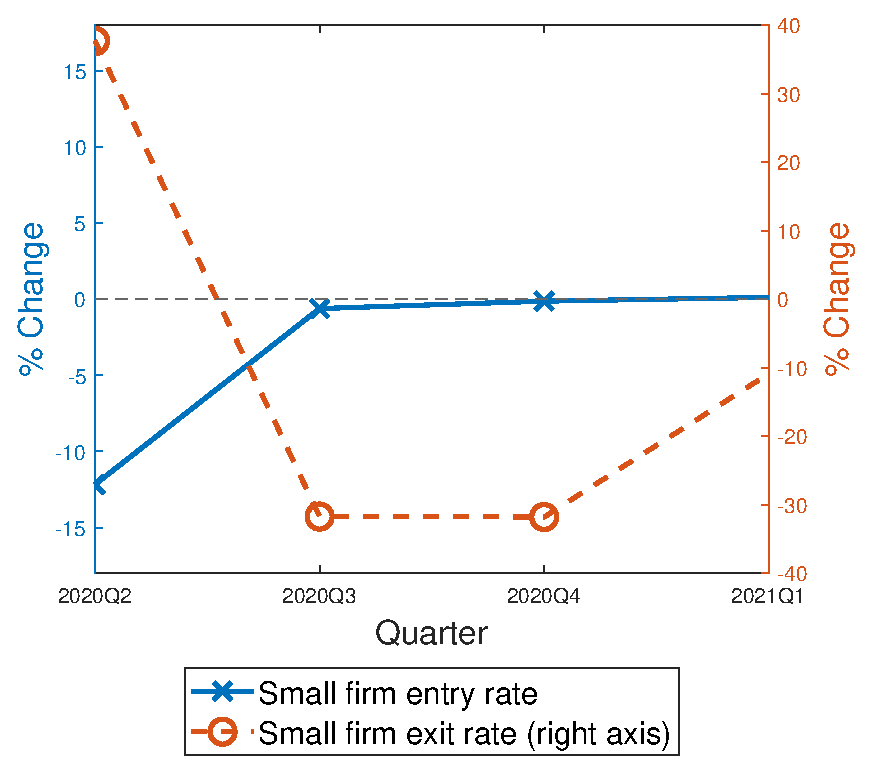
\includegraphics[width=\textwidth]{\FigDirGNG/model_mom_trans_bis}
		\caption{Transition of targeted aggregate variables in model}
	\end{subfigure}
\caption{Calibration of the pandemic shock}
\vspace{1ex}

\end{figure}

\FloatBarrier

\subsection{Results}


\begin{figure}[htbp]
	\centering
	\begin{subfigure}[b]{0.46\textwidth}
		\centering
		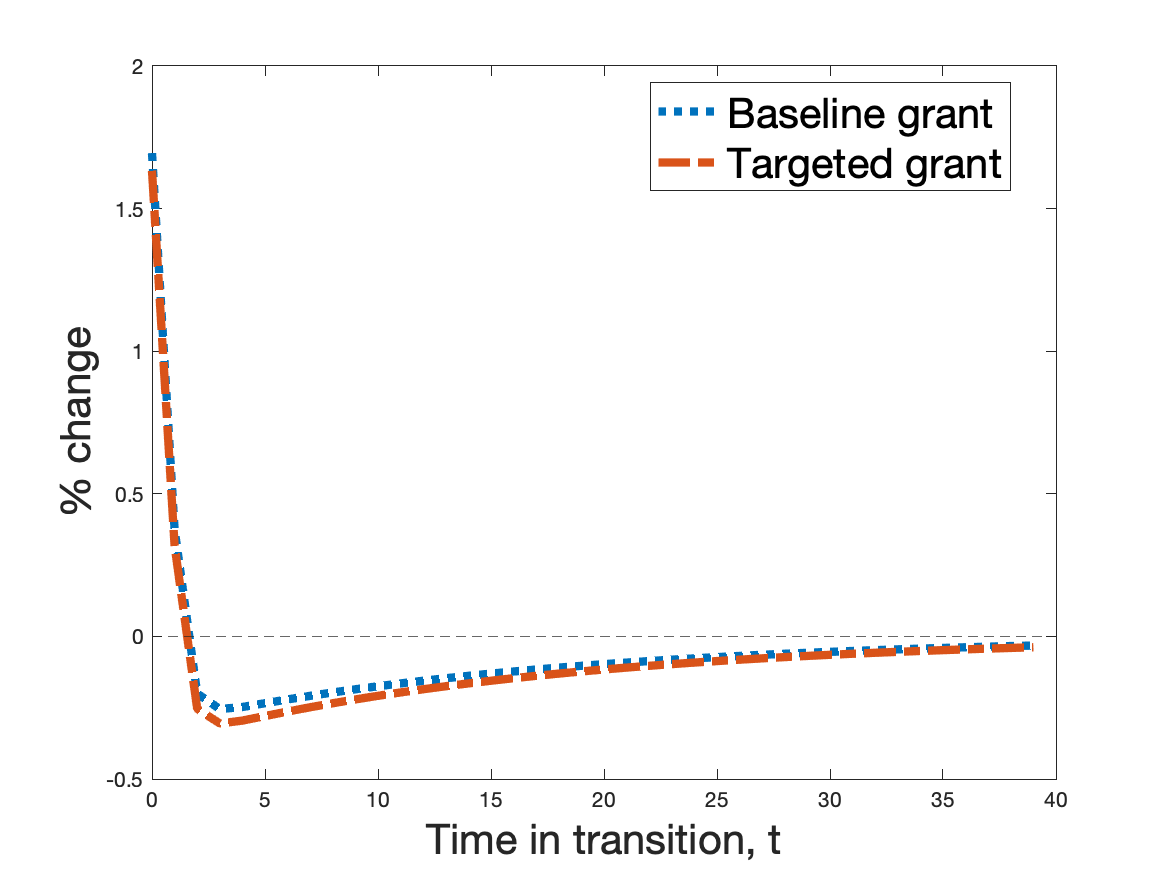
\includegraphics[width=\textwidth]{\FigDirGNG/irf_w}
		\caption{Wage, $ w_t $}
	\end{subfigure} \hfill
	\begin{subfigure}[b]{0.46\textwidth}
		\centering
		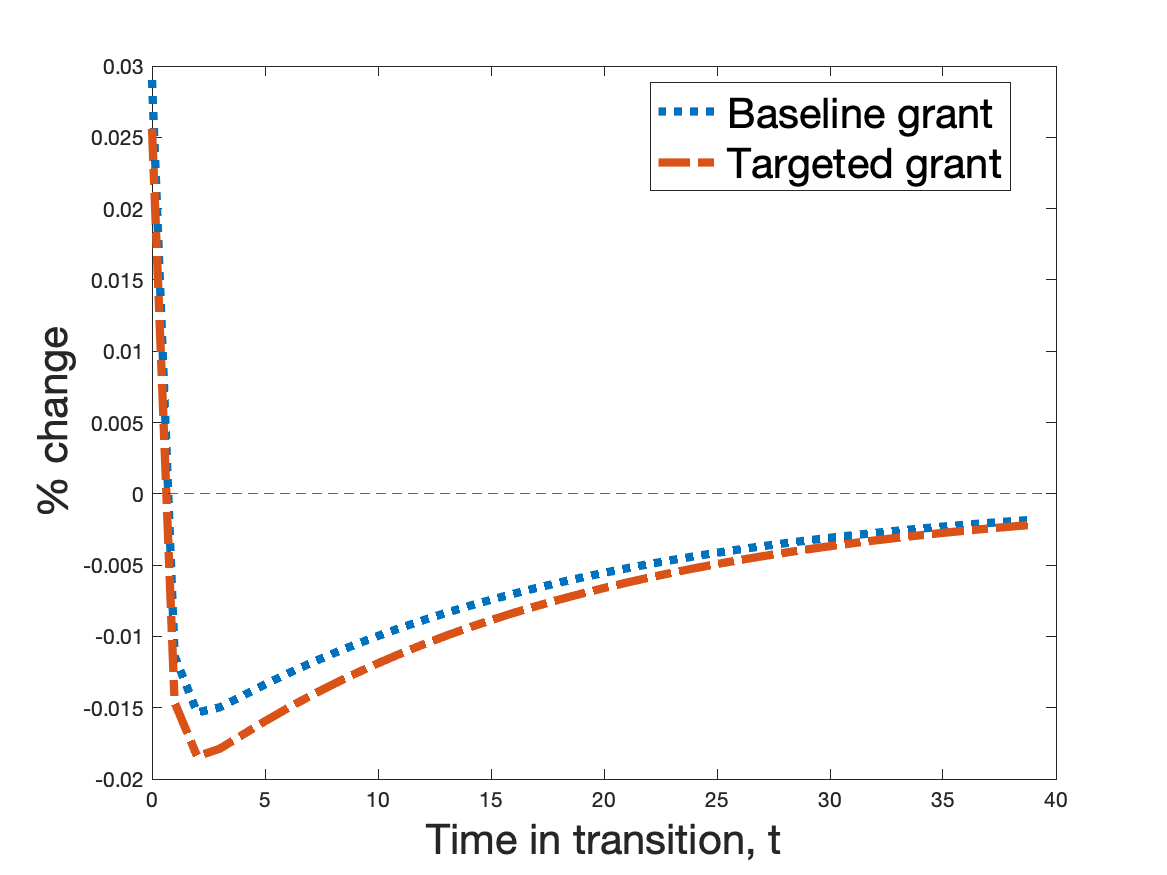
\includegraphics[width=\textwidth]{\FigDirGNG/irf_q}
		\caption{Financial discount factor, $ q_t $}
	\end{subfigure} 
	
	\caption{Responses to a pandemic shock: IRFs in each policy scenario}
	\label{fig:grant_vs_nogrant0}
\end{figure}
	
	\begin{figure}[htbp]
		\centering
		\begin{subfigure}[b]{0.46\textwidth}
			\centering
			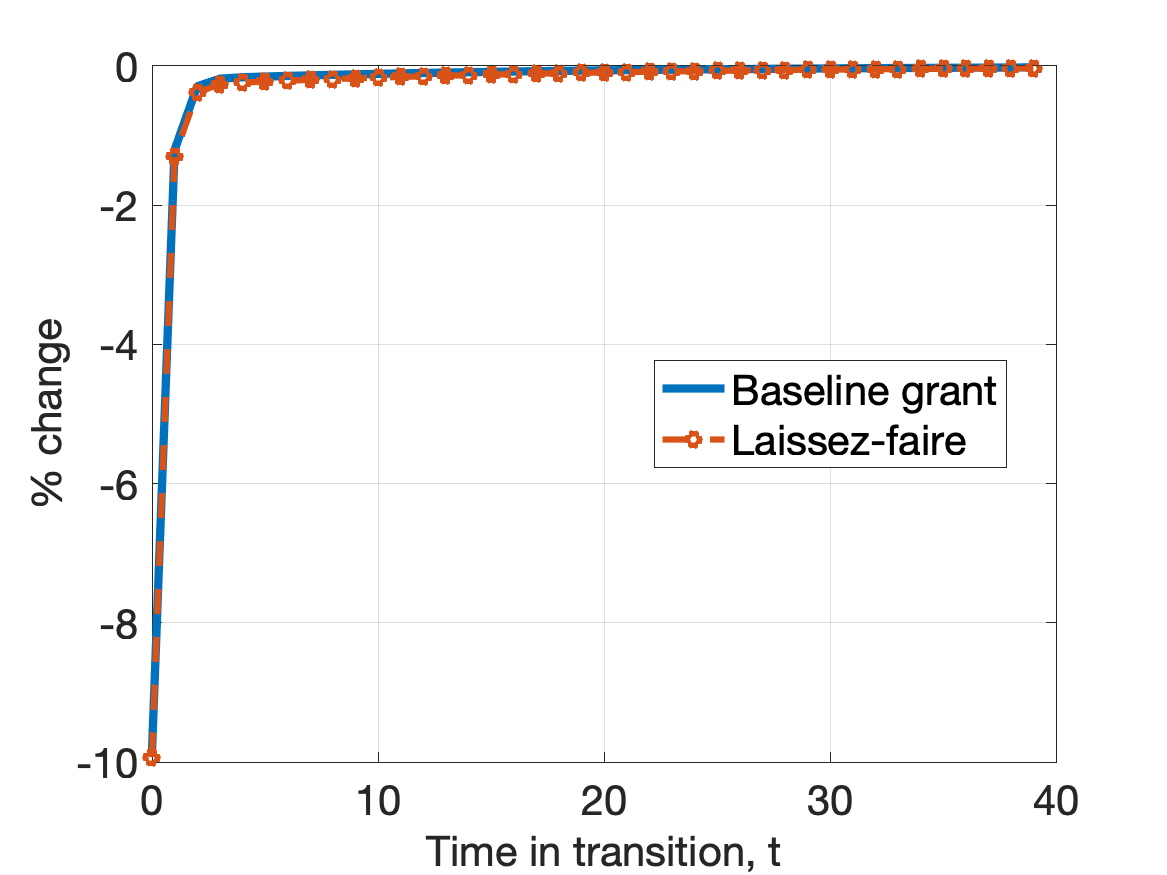
\includegraphics[width=\textwidth]{\FigDirGNG/irf_C_agg}
			\caption{Consumption}
		\end{subfigure} \hfill
		\begin{subfigure}[b]{0.46\textwidth}
			\centering
			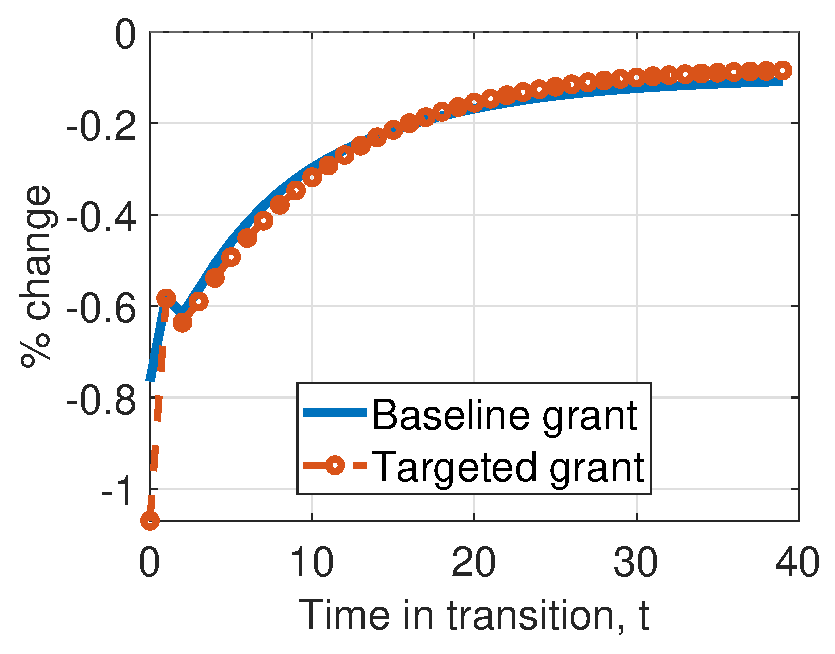
\includegraphics[width=\textwidth]{\FigDirGNG/irf_K_agg}
			\caption{Total capital, $ \tilde{K}_t $}
		\end{subfigure}
		\vskip\baselineskip
		\begin{subfigure}[b]{0.46\textwidth}
			\centering
			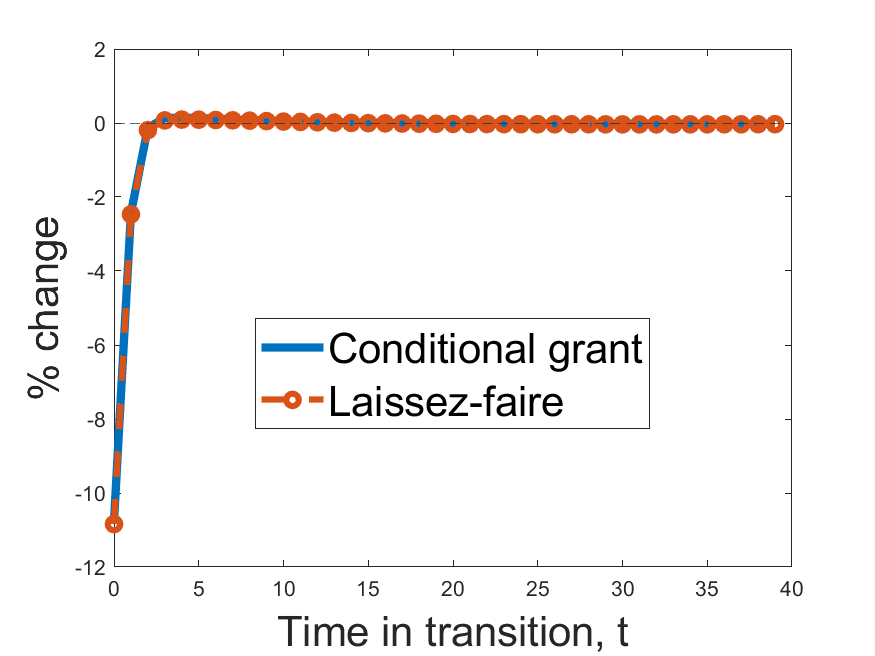
\includegraphics[width=\textwidth]{\FigDirGNG/irf_Y_agg}
			\caption{Total output}
		\end{subfigure}\hfill	
		\begin{subfigure}[b]{0.46\textwidth}
			\centering
			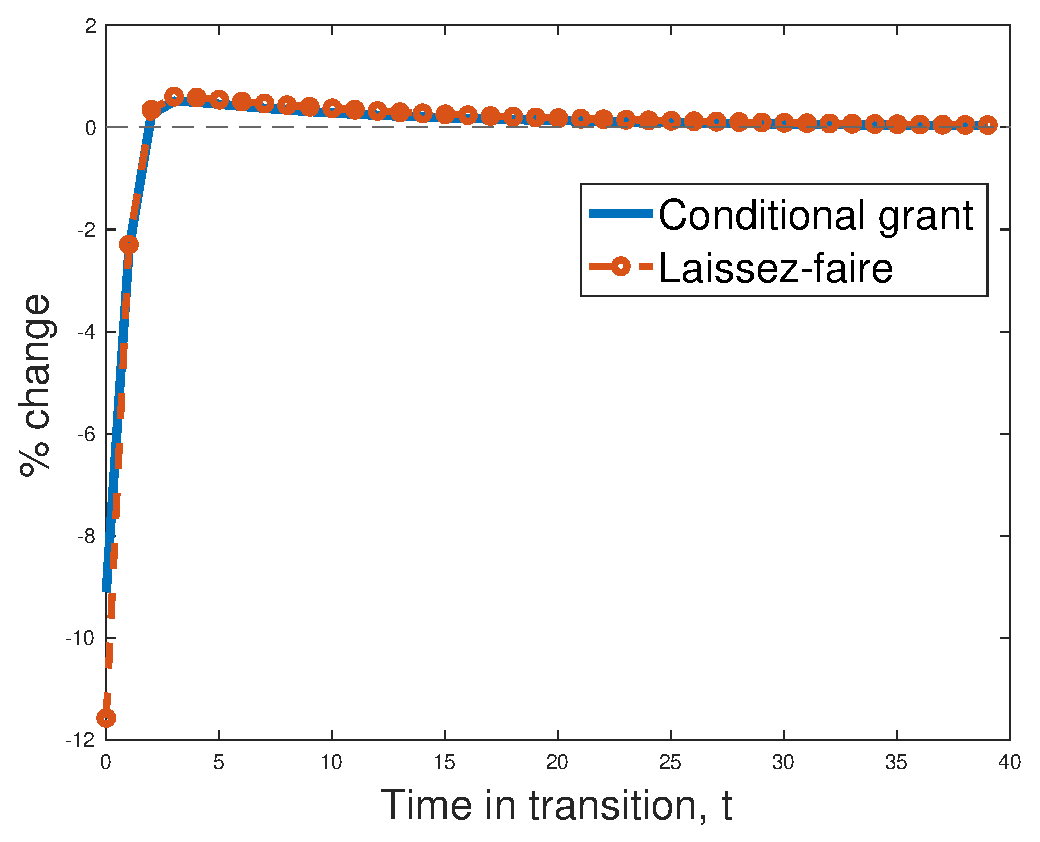
\includegraphics[width=\textwidth]{\FigDirGNG/irf_L_agg}
			\caption{Total employment}
		\end{subfigure} 
		\vskip\baselineskip
		\begin{subfigure}[b]{0.46\textwidth}
			\centering
			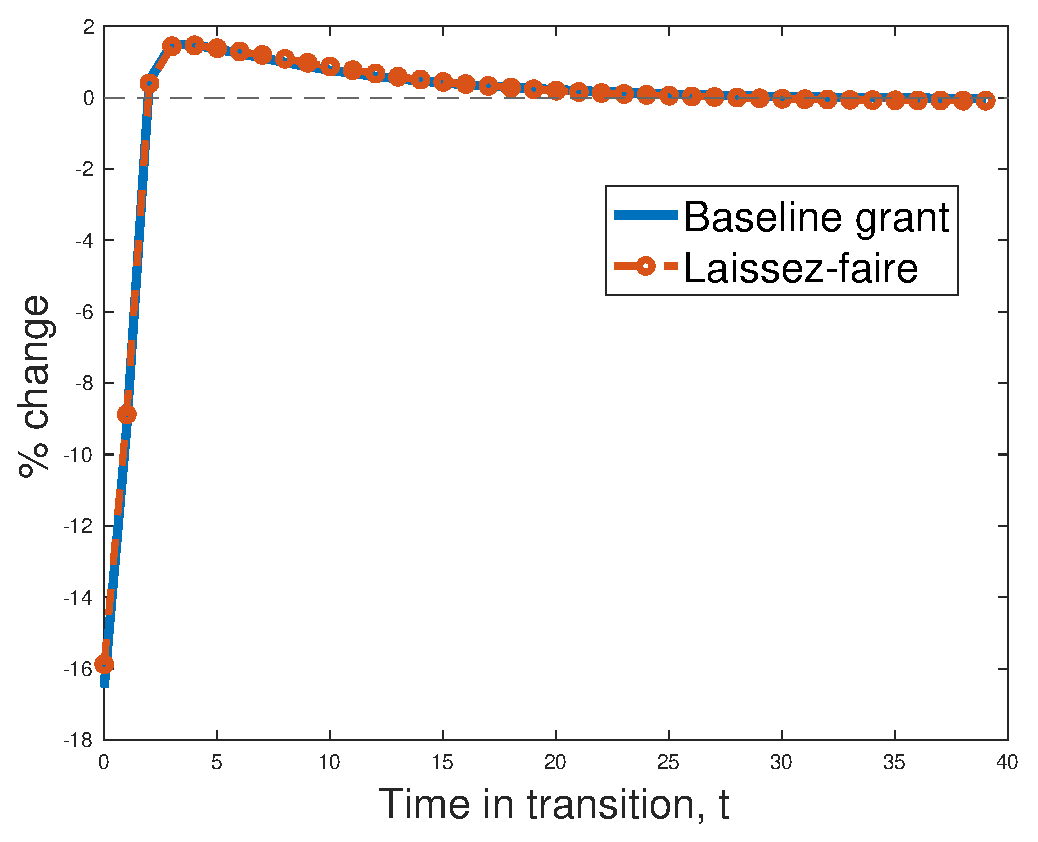
\includegraphics[width=\textwidth]{\FigDirGNG/irf_InvK}
			\caption{Total Investment}
		\end{subfigure} 
		\caption{Responses to a pandemic shock: IRFs in each policy scenario, cont'd}
		\label{fig:grant_vs_nogrant1}
	\end{figure}
		
	\begin{figure}[htbp]
		\centering	
		\begin{subfigure}[b]{0.46\textwidth}
			\centering
			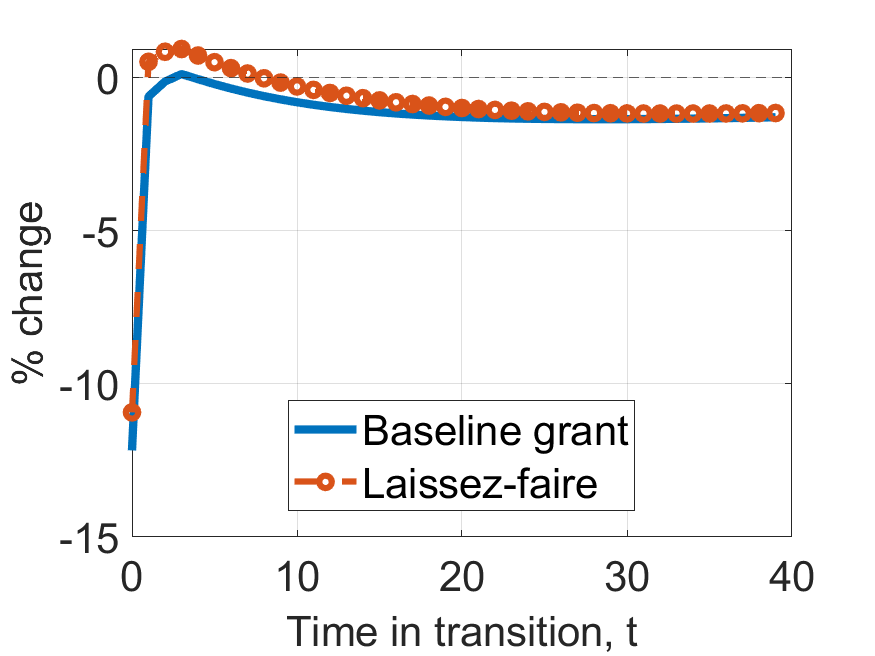
\includegraphics[width=\textwidth]{\FigDirGNG/irf_entry_rate}
			\caption{Entry rate}
		\end{subfigure} \hfill
		\begin{subfigure}[b]{0.46\textwidth}
			\centering
			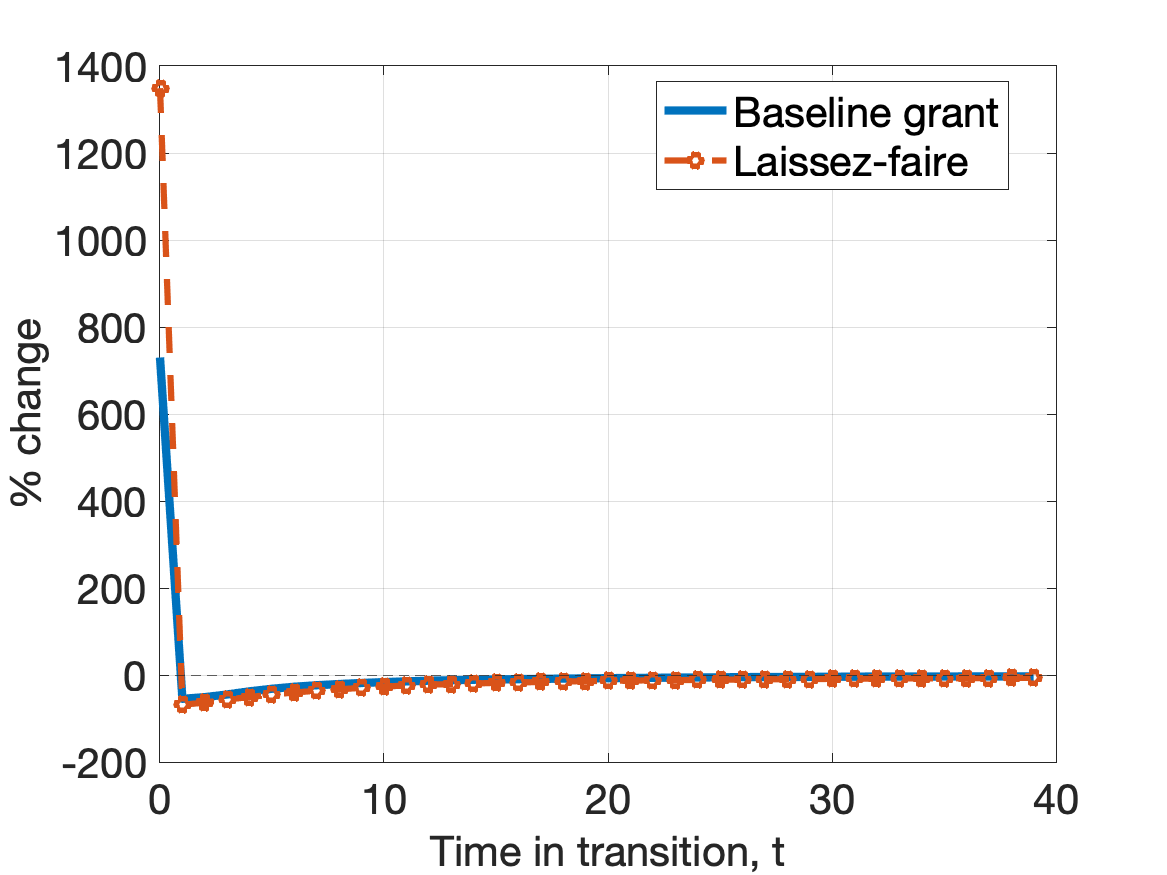
\includegraphics[width=\textwidth]{\FigDirGNG/irf_exit}
			\caption{Exit (measure of exiting firms)}
		\end{subfigure} 
		\vskip\baselineskip
		\begin{subfigure}[b]{0.46\textwidth}
			\centering
			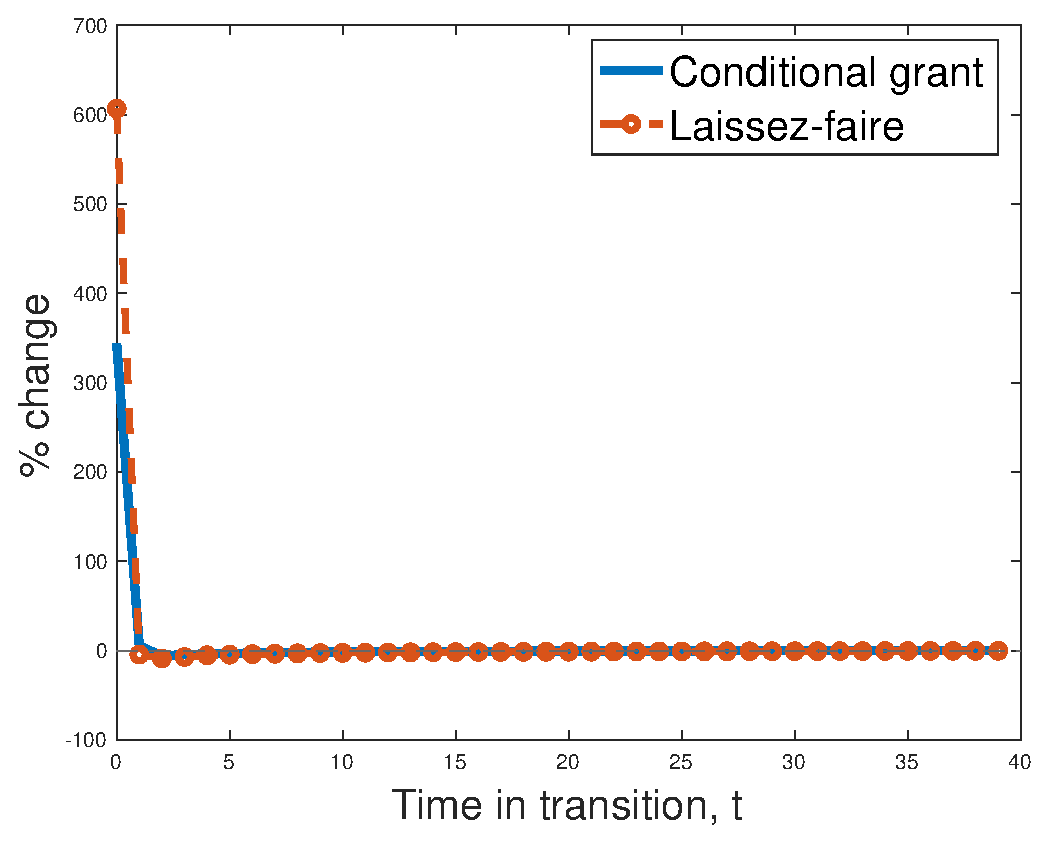
\includegraphics[width=\textwidth]{\FigDirGNG/irf_liq}
			\caption{Liquidation value of small firms}
		\end{subfigure} \hfill
		\begin{subfigure}[b]{0.46\textwidth}
			\centering
			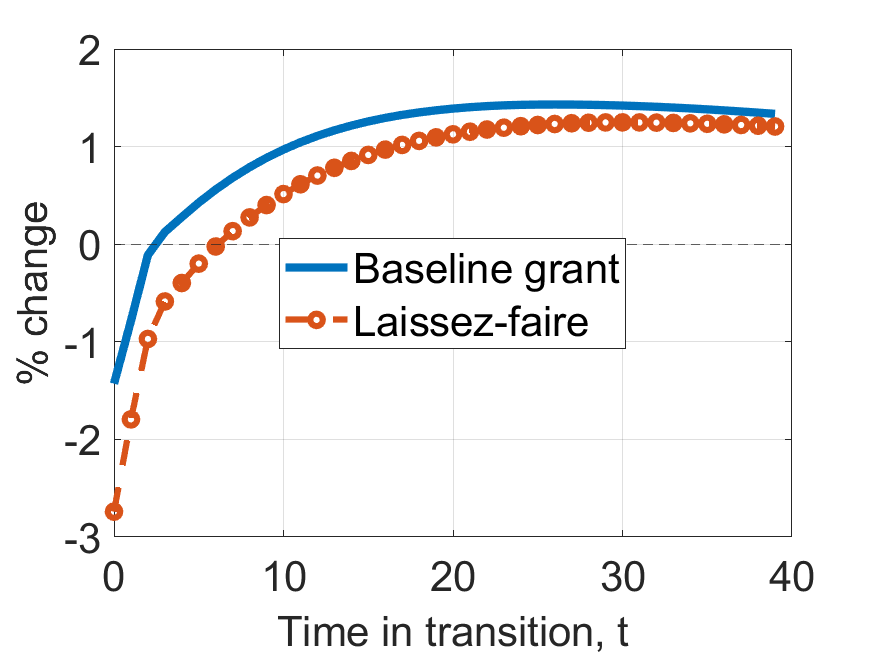
\includegraphics[width=\textwidth]{\FigDirGNG/irf_mass_small}
			\caption{Measure of small firms}
		\end{subfigure} 
		
		\caption{Responses to a pandemic shock: IRFs in each policy scenario, cont'd}
		\label{fig:grant_vs_nogrant2}
	\end{figure}		
		
		
	\begin{figure}[htbp]
		\centering
		\begin{subfigure}[b]{0.46\textwidth}
			\centering
			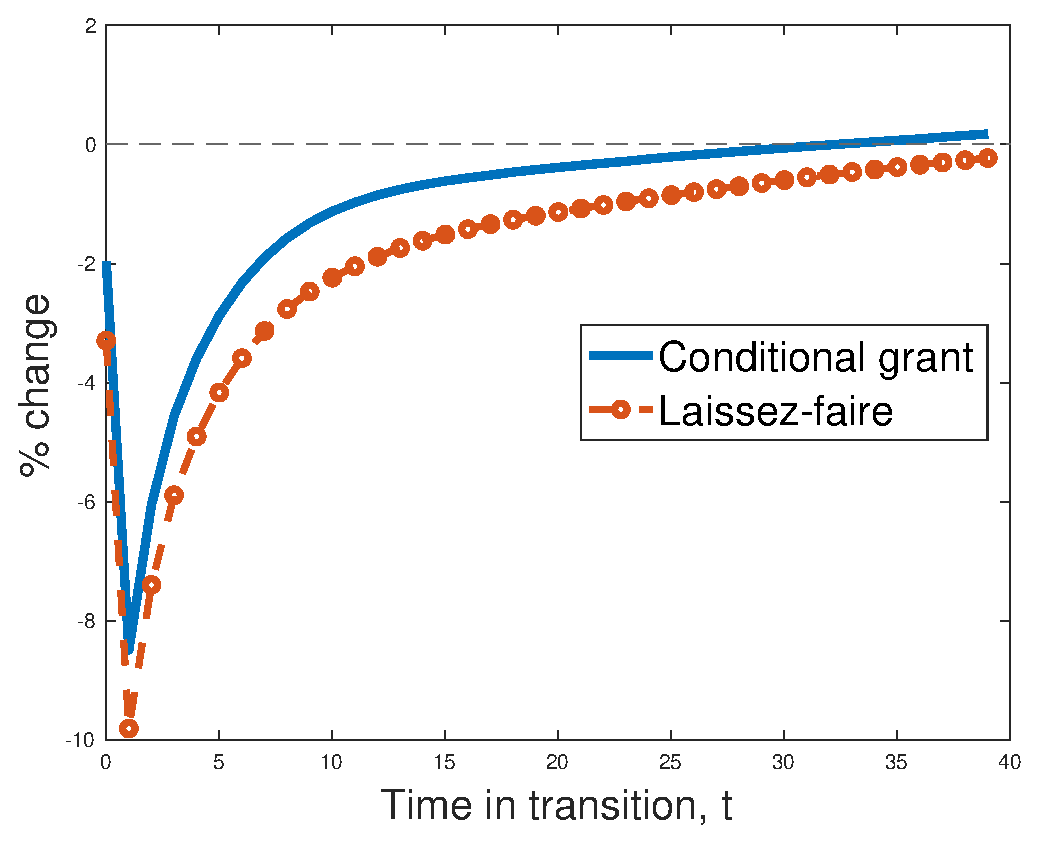
\includegraphics[width=\textwidth]{\FigDirGNG/irf_K_small}
			\caption{Capital, small firms}
		\end{subfigure} \hfill
		\begin{subfigure}[b]{0.46\textwidth}
			\centering
			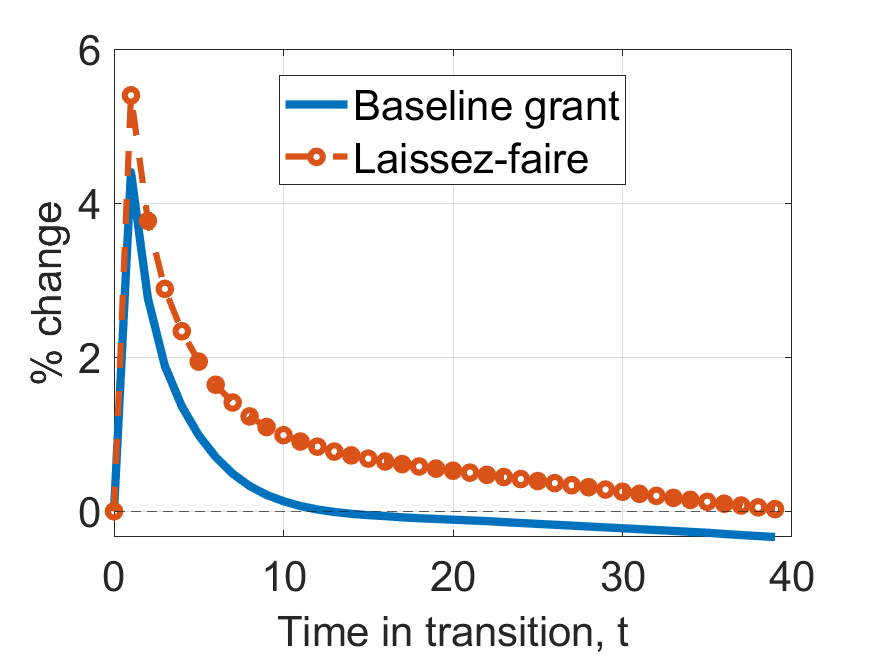
\includegraphics[width=\textwidth]{\FigDirGNG/irf_K_corp}
			\caption{Capital, corporate sector}
		\end{subfigure} \hfill
		\vskip\baselineskip
		\begin{subfigure}[b]{0.46\textwidth}
			\centering
			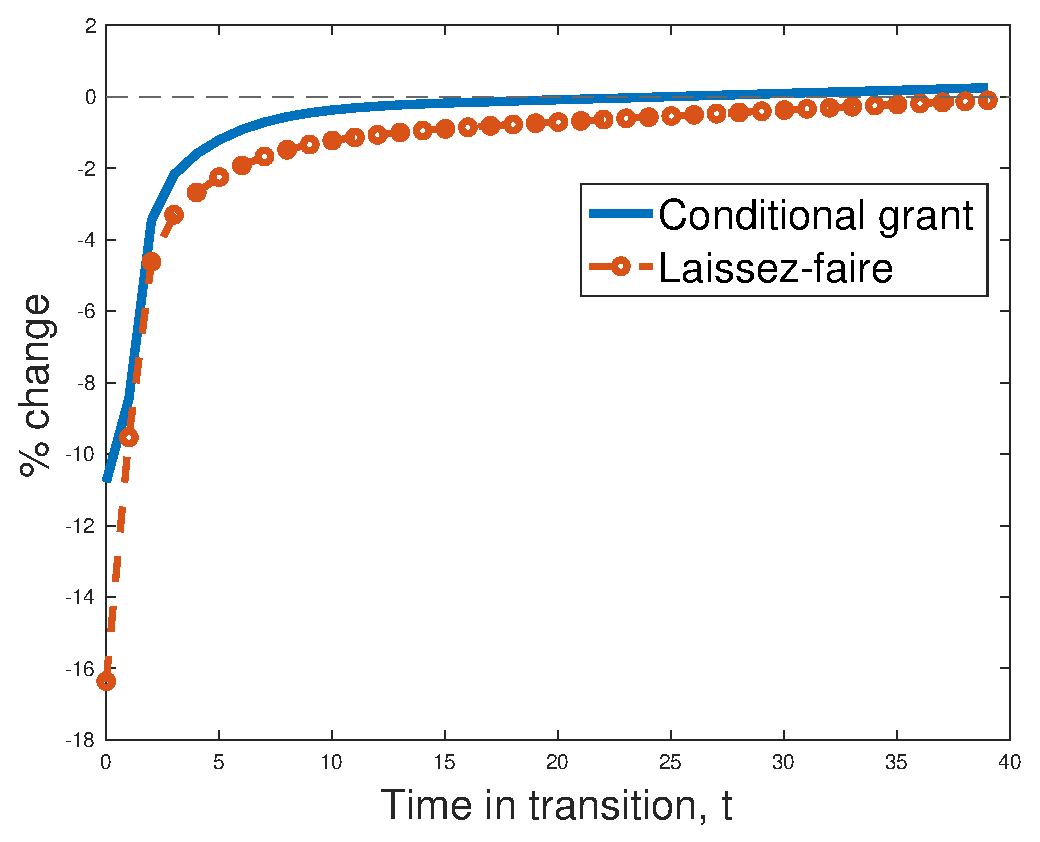
\includegraphics[width=\textwidth]{\FigDirGNG/irf_L_small}
			\caption{Employment, small firms}
		\end{subfigure} \hfill
		\begin{subfigure}[b]{0.46\textwidth}
			\centering
			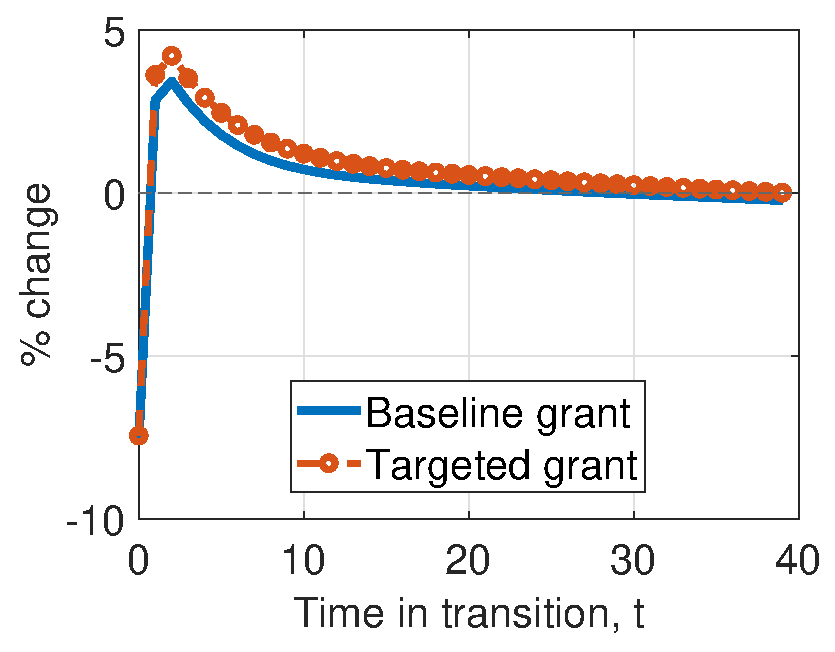
\includegraphics[width=\textwidth]{\FigDirGNG/irf_L_corp}
			\caption{Employment, corporate sector}
		\end{subfigure} 
		\vskip\baselineskip
		\begin{subfigure}[b]{0.46\textwidth}
			\centering
			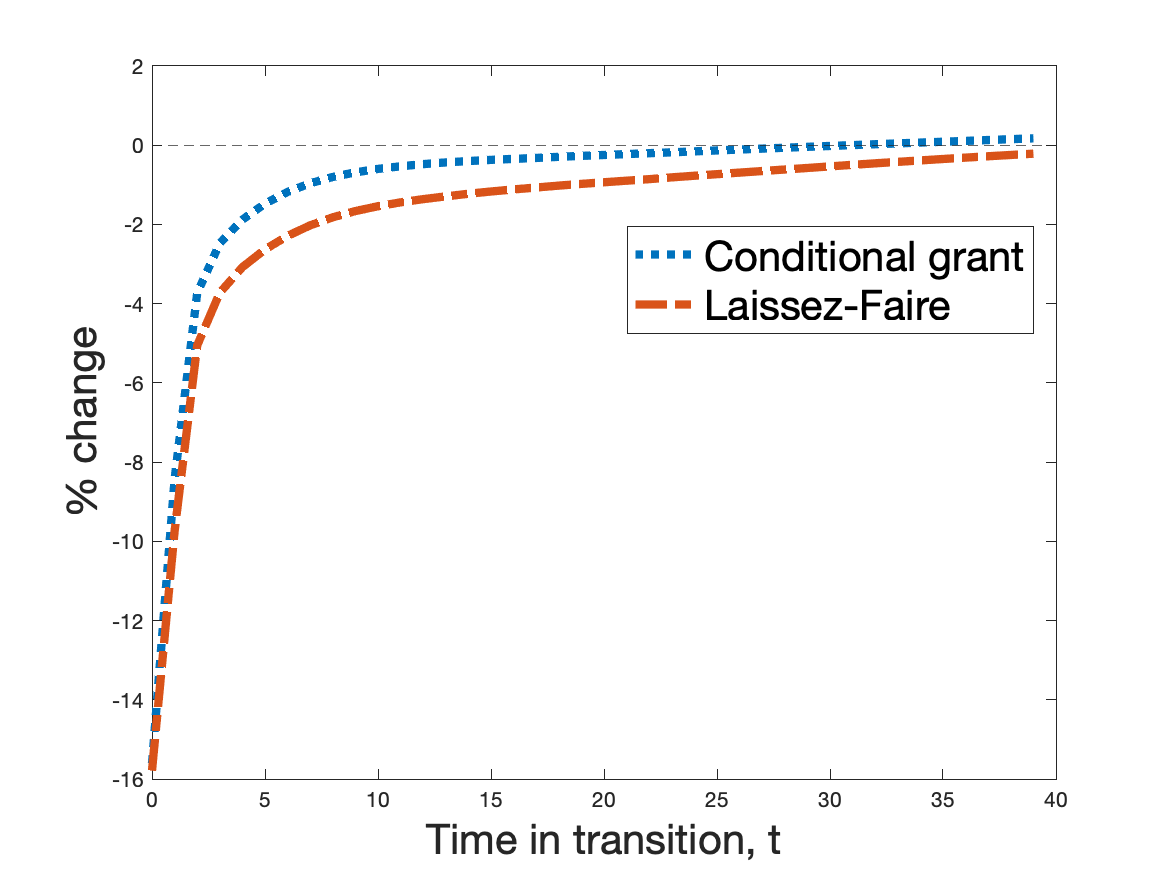
\includegraphics[width=\textwidth]{\FigDirGNG/irf_output_small}
			\caption{Output, small firms}
		\end{subfigure} \hfill
		\begin{subfigure}[b]{0.46\textwidth}
			\centering
			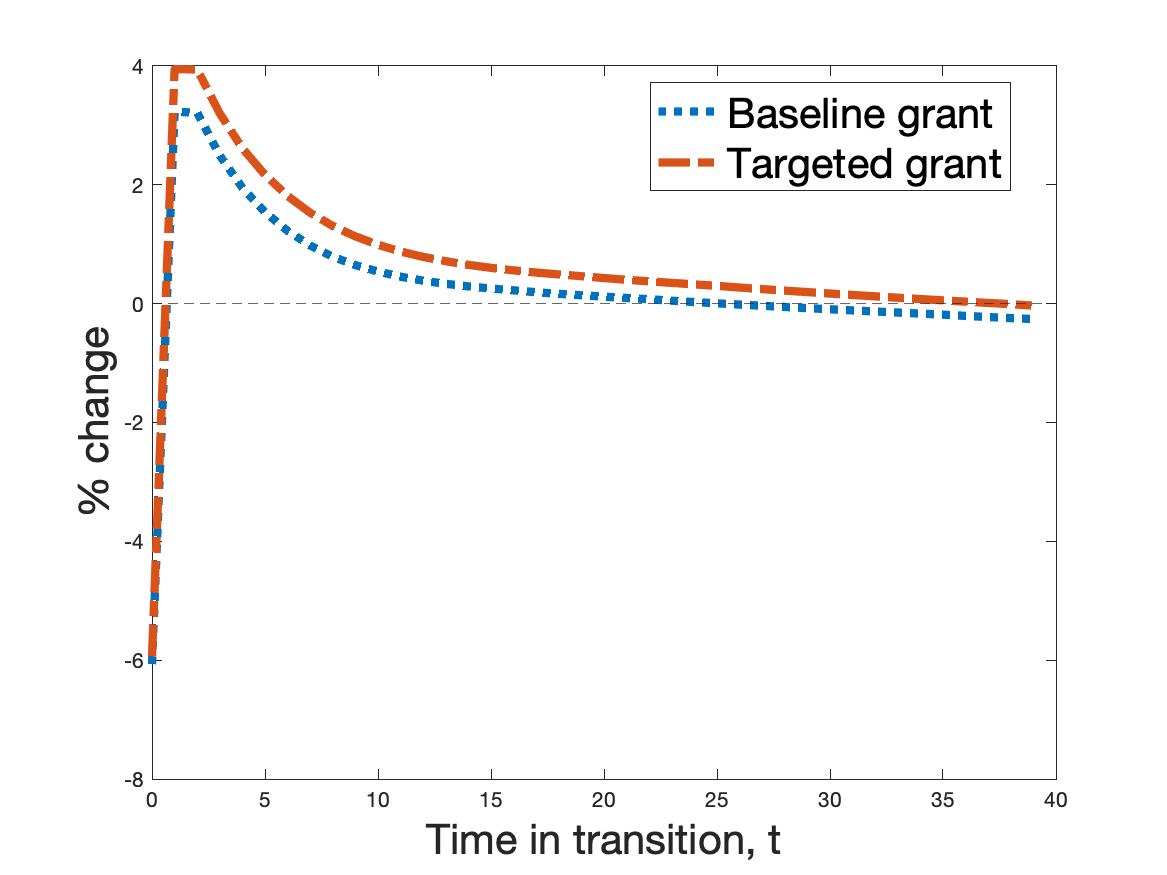
\includegraphics[width=\textwidth]{\FigDirGNG/irf_Y_corp}
			\caption{Output, corporate sector}
		\end{subfigure} 
			
		\caption{Responses to a pandemic shock: IRFs in each policy scenario, cont'd}
		\label{fig:grant_vs_nogrant3}
	\end{figure}		

	
	\begin{figure}[htbp]
		\centering
		\begin{subfigure}[b]{0.46\textwidth}
			\centering
			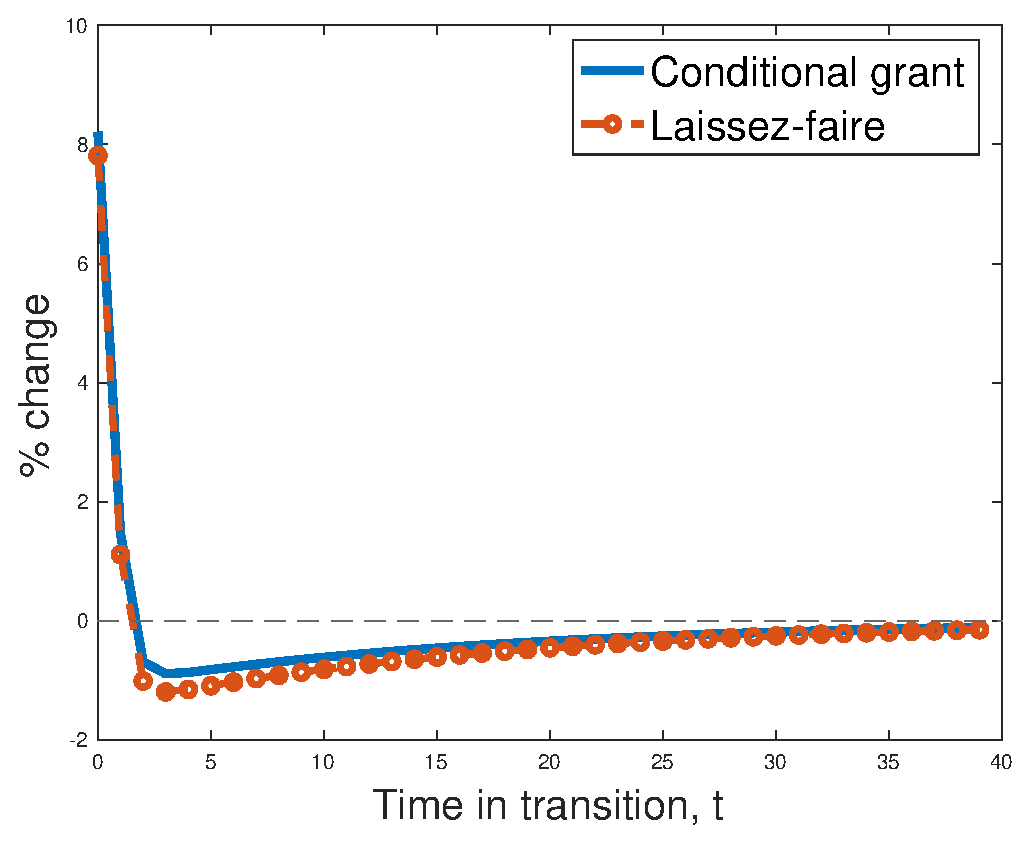
\includegraphics[width=\textwidth]{\FigDirGNG/irf_KL_ratio}
			\caption{Capital-to-Labor ratio, corporate, sector}
		\end{subfigure} \hfill
		\begin{subfigure}[b]{0.46\textwidth}
			\centering
			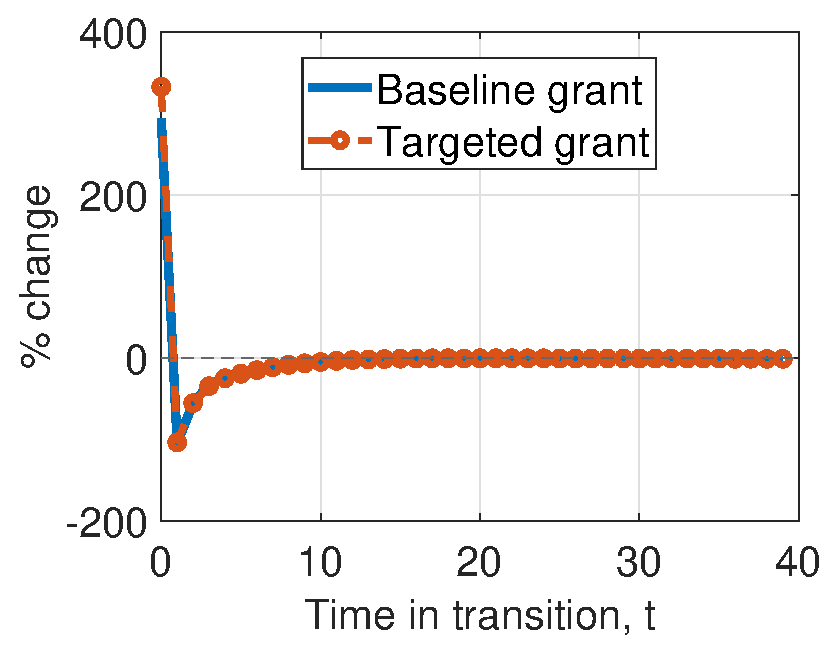
\includegraphics[width=\textwidth]{\FigDirGNG/irf_InvK_corp}
			\caption{Investment, corporate sector}
		\end{subfigure} 

		\caption{Responses to a pandemic shock: IRFs in each policy scenario, cont'd}
		\label{fig:grant_vs_nogrant4}
	\end{figure}

    \begin{figure}[htbp]
    	\centering
    		\centering
    		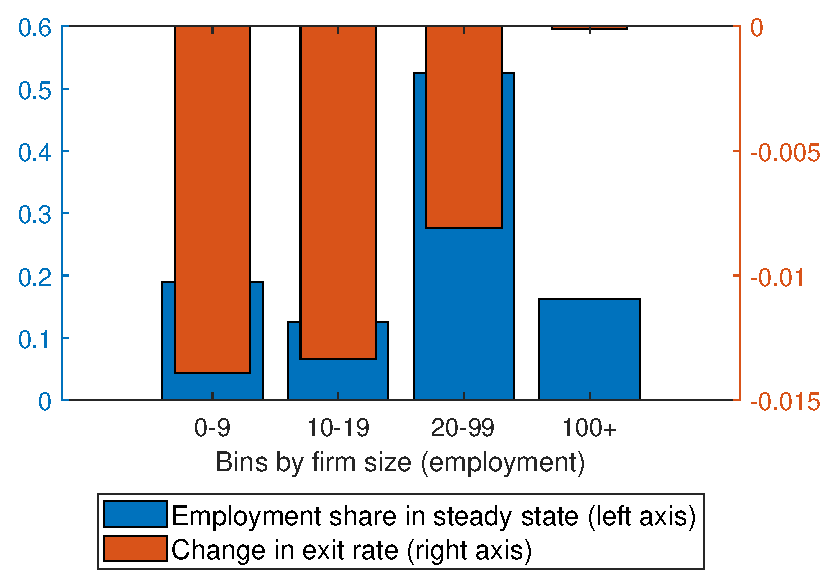
\includegraphics[width=0.8\textwidth]{\FigDirGNG/emp_exit_rate_lbins}
    		\caption{Employment share by deciles of firm size and change in exit rate due to  grant}

\vspace{1ex}
	{\textit{Notes:} \raggedright Average firm size in the first bin is ? \par} 
 
    \end{figure}

\FloatBarrier
	
\subsection{Policy effects on small firm investments}
In addition to saving small firms from a total liquidation, the rescue grant
also plays a role in firms' investment decisions. The pandemic shocks may
force small firms to liquidate part of their capital in order to pay a
non-negative dividend. Due to the partial irreversibility of capital, such
liquidation may be inefficient. The rescue policy can prevent firms from
liquidating their capital. For firms that are unimpacted and not forced to
liquidate their capital, the rescue grant may lead to an increase in capital
investment. We quantify the impact of the rescue policy on investment by
compute the amount of inefficient capital liquidation prevented and the
amount of additional investment boosted by the policy.

There are in total four types of capital adjustments: upward and downward
adjustments by active firms, capital buying by entrants, and capital selling
by exiters. We compute the aggregate value of adjustments. 

\begin{itemize}
\item Upward capital adjustment by active firms: 
\begin{equation*}
\mathcal{A}_u = \int k^{\prime }_u(x,b,k) d\mu(x,b,k)
\end{equation*}
where $k^{\prime }_u(x,b,k) \equiv \max \{k^{\prime }(x,b,k)-(1-\delta)k,0 \}
$.

\item Downward capital adjustment by active firms: 
\begin{equation*}
\mathcal{A}_d = \int k^{\prime }_d(x,b,k) d\mu(x,b,k)
\end{equation*}
where $k^{\prime }_d(x,b,k) \equiv \min \{k^{\prime }(x,b,k)-(1-\delta)k,0 \}
$.

\item Capital bought by entrants: 
\begin{equation*}
\mathcal{A}_{ue} = M \int k d^e(x,b,k) d\Phi(x,b,k).
\end{equation*}

\item Capital sold by exiters: 
\begin{equation*}
\mathcal{A}_{de} = -\int k (\psi + (1-\psi)d^l(x,b,k)) d\mu^0(x,b,k).
\end{equation*}
\end{itemize}

We can also compute the counterparts of the above for each period on the
transition path and compare them to the steady state. For each $t$ on the transition path, we can compute the four types of capital adjustment as follows:

\begin{itemize}
\item Upward capital adjustment by active firms: 
\begin{equation*}
\mathcal{A}_{u,t+1} = \int k^{\prime }_{u,t}(x,b,k) d\mu_{t}(x,b,k)
\end{equation*}
where $k^{\prime }_{u,t}(x,b,k) \equiv \max \{k^{\prime }_t(x,b,k)-(1-\delta)k,0 \}$. Note that for $K^{\prime }_{u,t=0} = K^{\prime }_{u}$, the steady state value. This is because capital of continuing firms in $t=0$ is determined by the investment decisions made in the previous period, before the pandemic shock hits the economy.

\item Downward capital adjustment by active firms: 
\begin{equation*}
\mathcal{A}_{d,t+1} = \int k^{\prime }_{d,t}(x,b,k) d\mu_{t}(x,b,k)
\end{equation*}
where $k^{\prime }_{d,t}(x,b,k) \equiv \min \{k^{\prime }_t(x,b,k)-(1-\delta)k,0 \}$. Note that for $K^{\prime }_{d,t=0} = K^{\prime }_{d}$, the steady state value.

\item Capital bought by entrants: 
\begin{equation*}
\mathcal{A}_{ue,t} = M_t \int k d^e_t(x,b,k) d\Phi(x,b,k).
\end{equation*}

\item Capital sold by exiters: 
\begin{equation*}
\mathcal{A}_{de,t} = -\int k (\psi + (1-\psi)d^l_t(x,b,k)) d\mu^0_t(x,b,k).
\end{equation*}

\end{itemize}

In Table \ref{tab:capadj_ss}, we compute steady state capital adjustment rates, which are defined as capital adjustments divided by the steady state capital in the small firm sector. 

Figure \ref{fig:capadj} shows the paths of capital adjustments. The capital adjustments in these graphs are shown as a percentage of the steady state capital in the small firm sector. 

Next, we decompose cumulative changes in small firm capital in the pandemic into the four types of capital adjustments. We consider the following time spans: (a) Short run: change from the pre-pandemic time to the end of Q2; (b) medium run: Q3-Q8; (c) long run: Q9-Q40; (d) Q1-Q40. We show the results in Figure \ref{fig:capadj_bar}. 
For example, consider the upward capital adjustment by small firms. We compute the cumulative excess upward adjustment in each time span as follows:

\begin{itemize}
\item Short run:
\begin{equation*}
\Delta \mathcal{A}_{u,sr} = \sum_{t=1}^{T_{sr}} \left( \mathcal{A}_{u,t} -  \mathcal{A}_{u}  \right)
\end{equation*}
\item Medium run:
\begin{equation*}
\Delta \mathcal{A}_{u,mr} = \sum_{t=T_{sr}+1}^{T_{mr}} \left( \mathcal{A}_{u,t} -  \mathcal{A}_{u}  \right)
\end{equation*}
\item Long run:
\begin{equation*}
\Delta \mathcal{A}_{u,lr} = \sum_{t=T_{mr}+1}^{T_{lr}} \left( \mathcal{A}_{u,t} -  \mathcal{A}_{u}  \right)
\end{equation*}
\item Overall:
\begin{equation*}
\Delta \mathcal{A}_{u,all} = \sum_{t=1}^{T_{lr}} \left( \mathcal{A}_{u,t} -  \mathcal{A}_{u}  \right)
\end{equation*}
\end{itemize}
In Figure \ref{fig:capadj_bar}, we express the cumulative excess capital adjustments as a percentage of the steady state capital in small firms. For example, we plot $\frac{\Delta \mathcal{A}_{u,sr}}{K_{small}}$ in panel A. In the figure, we also plot the sum of all four types of excess capital adjustments. For example, the sum in the short run is equal to $\Delta \mathcal{A}_{u,sr} + \Delta \mathcal{A}_{d,sr} +\Delta \mathcal{A}_{ue,sr} +\Delta \mathcal{A}_{de,sr}$.

\begin{table}[htbp]
	\caption{Four types of capital adjustment rates in the steady state}
   	\label{tab:capadj_ss}
   	\centering
   	 \begin{tabular}{lc} \hline \hline 
Up. adj. by active firms &    0.056 \\ 
Down. adj. by active firms &   -0.052 \\ 
Capital bought by entrants &    0.015 \\ 
Capital sold by exiters &   -0.004 \\ 
Overall small-firm investment rate &    0.015 \\ 
\hline \hline 
 \end{tabular} 

   	\vspace{1ex}
   	
   	{\textit{Notes:} \raggedright  Capital adjustment rates and the overall investment rate are computed relative to steady state small firm capital. 
   	\par}
\end{table}

\begin{figure}[htbp]
		\centering
		\begin{subfigure}[b]{0.46\textwidth}
			\centering
			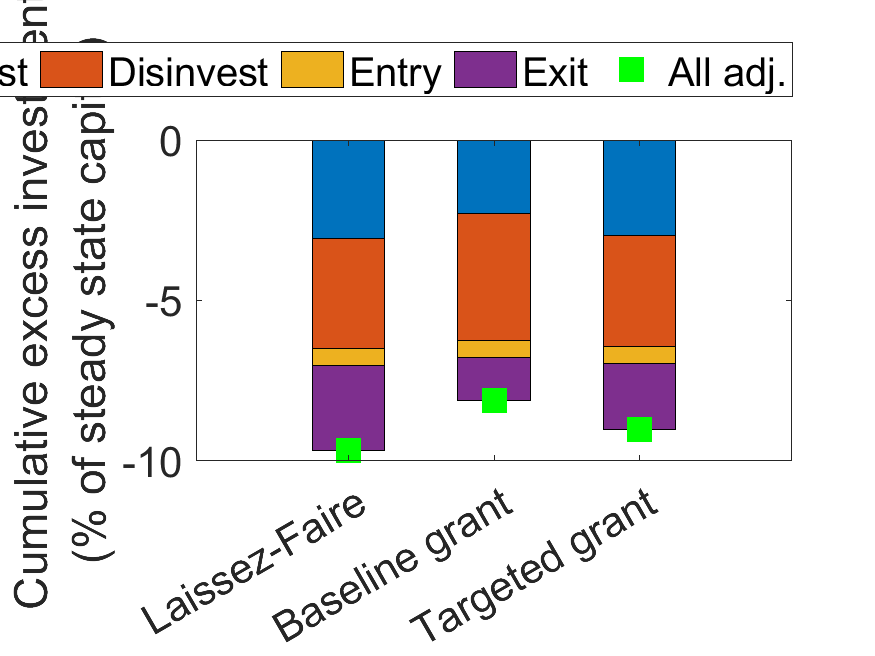
\includegraphics[width=\textwidth]{\FigDirGNG/cum_capadj_decomp_sr}
			\caption{Short run: Q1-Q2}
		\end{subfigure} \hfill
		\begin{subfigure}[b]{0.46\textwidth}
			\centering
			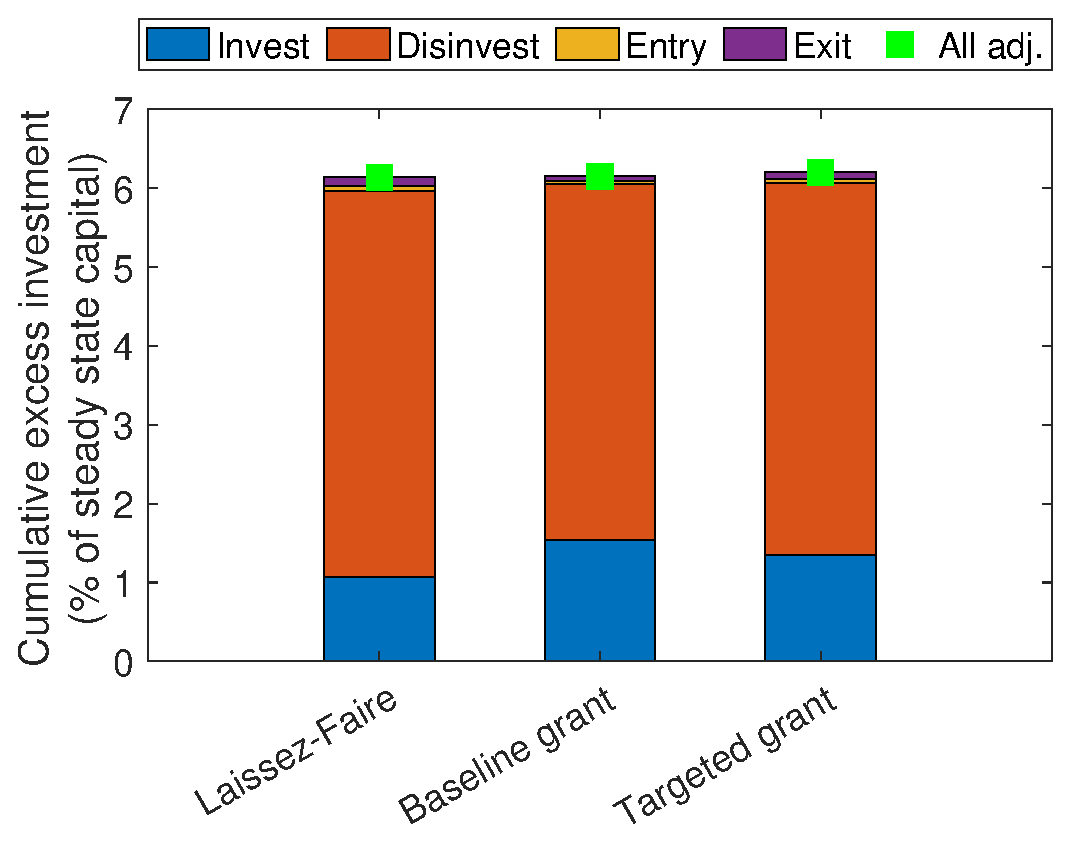
\includegraphics[width=\textwidth]{\FigDirGNG/cum_capadj_decomp_mr}
			\caption{Medium run: Q3-Q8}
		\end{subfigure} 
		\vskip\baselineskip
\begin{subfigure}[b]{0.46\textwidth}
			\centering
			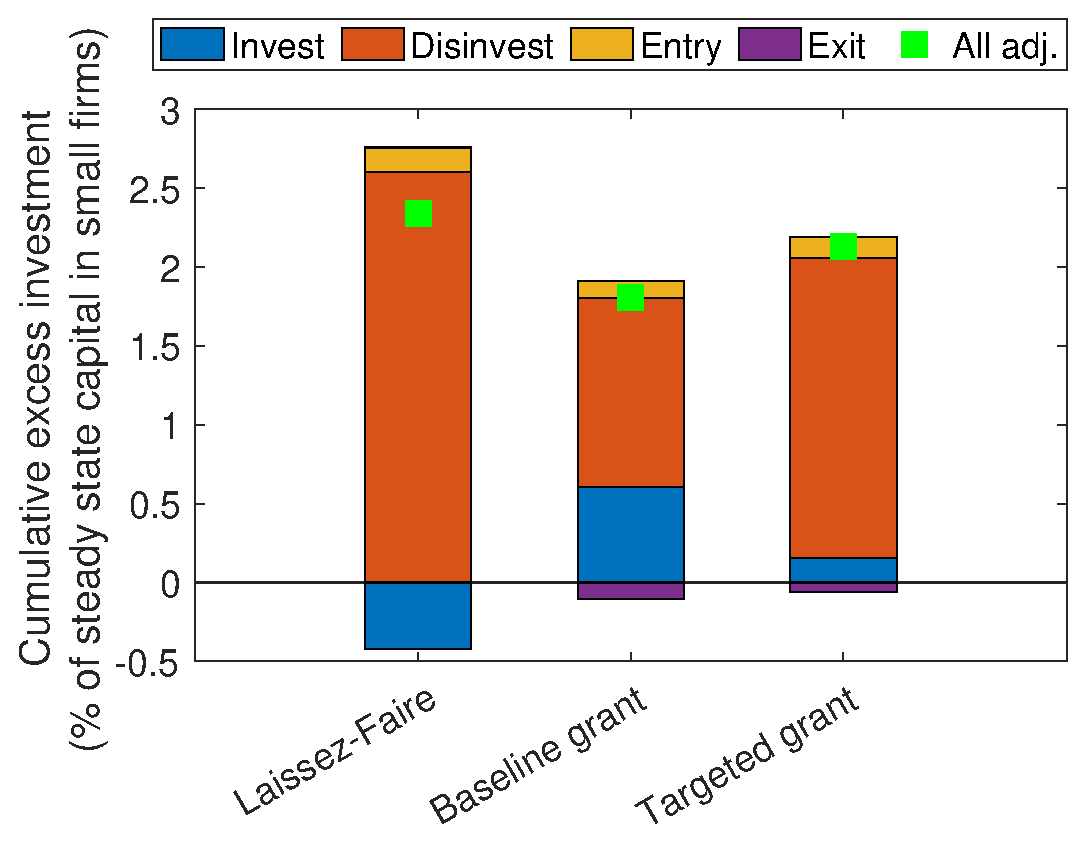
\includegraphics[width=\textwidth]{\FigDirGNG/cum_capadj_decomp_lr}
			\caption{Long run: Q9-Q40}
		\end{subfigure} \hfill
		\begin{subfigure}[b]{0.46\textwidth}
			\centering
			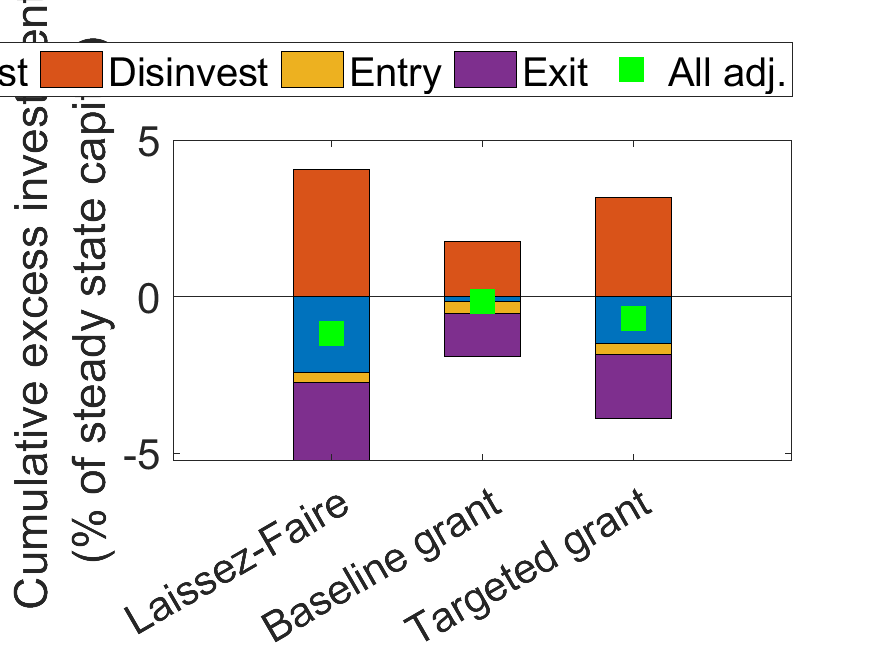
\includegraphics[width=\textwidth]{\FigDirGNG/cum_capadj_decomp_all}
			\caption{Q1-Q40}
		\end{subfigure} 
		\caption{Cumulative excess investment by types of capital adjustment}
		\label{fig:capadj_bar}
		
		\vspace{1ex}
		
		{\textit{Notes:} \raggedright Invest. = upward capital adjustment by active firms; Disinvest. = downward capital adjustment by active firms; Entry = capital bought by entrants; Exit = capital sold by exiters.    \par}		
		
	\end{figure}
	
\FloatBarrier


\subsection{Firm indebtedness}


On the transition path, the firm exit rate drops below the steady state level after the initial impact in both the baseline economy and the laissez-faire economy. To understand why the exit rate drops, it is helpful to look at changes in firm indebtedness on the transition path. Figure \ref{fig:firmdebt} shows that firms are on average less indebted in both policy scenarios. Partly this is because of the credit shock, which tightens the debt limit of firms. 
There are also reasons specific to each policy scenario that lead to a decrease in firm indebtedness.
In the baseline economy, firms are less indebted because of the grant. In the laissez-faire economy, many highly indebted firms exit on impact and continuing firms make less capital investment (see  Figure \ref{fig:capadj} (a)).

%From Figure \ref{fig:capadj}, we can see that, in the laissez-faire economy, stayers downward adjust capital significantly upon impact and there is less upward adjustment of capital by stayers. 

\begin{figure}[htbp]
	\centering
	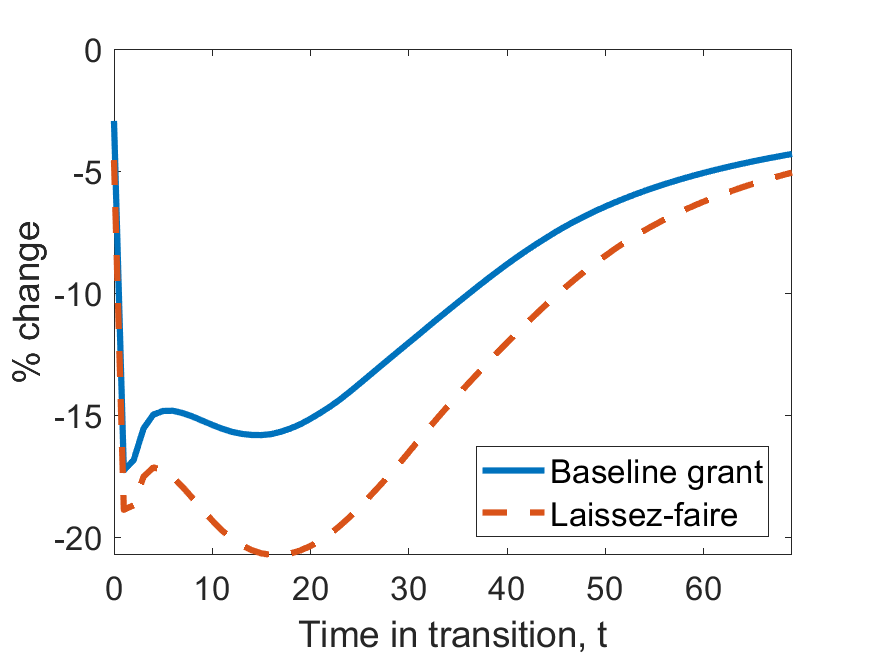
\includegraphics[scale=0.7]{\FigDirGNG/irf_ave_bk}
		
	\caption{Firm indebtedness}
	\label{fig:firmdebt}
\end{figure}
	
\FloatBarrier
	
\subsection{Zombie firms}

\begin{table}[htbp]
	 \begin{tabular}{lc} \hline \hline 
Baseline grant & \\ 
Fraction of saved firms &   0.4713 \\ 
Fraction of zombie firms &   0.0135 \\ 
\hline 
Targeted grant & \\ 
Fraction of saved firms &   0.6850 \\  
Fraction of zombie firms &   0.0036 \\ 
Targeted grant (large) & \\ 
Fraction of saved firms &   0.8979 \\  
Fraction of zombie firms &   0.0180 \\ 
\hline \hline 
 \end{tabular} 

	\caption{Zombie firm analysis. Impact period only.}
		
    \vspace{1ex}
    {\textit{Notes:} \raggedright Fraction of saved firms is the measure of saved firms in period $t=0$ divided by the measure of firms that exit under the laissez-faire environment, all conditional on receiving the grant. Fraction of zombie firms is the measure of zombie firms divided by the measure of saved firms.    \par}		
\end{table}	

\FloatBarrier

\subsection{Welfare analysis}	
	Inputs: Let $C_{ss}$ and $L_{ss}$ denote consumption and employment in the
steady-state. Let $\left\{ C_{t},L_{t}\right\} _{t=1}^{T+1}$ denote
consumption and labor along the transition. We assume that the economy has
reached the steady-state for $t\geq T+2$.

The utility function is%
\begin{equation*}
U(C,L)=\frac{C^{1-\sigma }}{1-\sigma }+\zeta (1-L).
\end{equation*}%
During the transition it is%
\begin{equation*}
U(C_{t},L_{t};D_t,\zeta _{t})=\frac{D_t C_{t}^{1-\sigma }}{1-\sigma }+\zeta
_{t}\zeta(1-L_{t})
\end{equation*}%
The value in the steady-state is%
\begin{equation*}
V_{ss}=\frac{1}{1-\beta }U(C_{ss},L_{ss})=\frac{1}{1-\beta }\left[ \frac{%
C_{ss}^{1-\sigma }}{1-\sigma }+\zeta (1-L_{ss})\right] =V_{ss}^{C}+V_{ss}^{L}
\end{equation*}%
where $V_{ss}^{C}=\frac{1}{1-\beta }\frac{C_{ss}^{1-\sigma }}{1-\sigma }$
and $V_{ss}^{L}=\frac{1}{1-\beta }\zeta (1-L_{ss})$.

The value in the first period of the transition is%
\begin{align*}
V_{t=1}=&U(C_{1},L_{1};D_1,\zeta _{1})+\beta U(C_{2},L_{2};D_2,\zeta _{2})+\ldots
+\beta ^{T}U(C_{T+1},L_{T+1};D_{T+1},\zeta _{T+1}) \\
& +\sum_{j=T+2}^{\infty }\beta
^{j-1}U(C_{j},L_{j};D_j,\zeta _{j})
\end{align*}%
where $C_{j}=C_{ss}$, $L_{j}=L_{ss}$, $D_j = 1$ and $\zeta_j=1$ for all $j\geq T+2$. Therefore the
equation above can be simplified to 
\begin{equation*}
V_{t=1}=U(C_{1},L_{1};D_1,\zeta _{1})+\beta U(C_{2},L_{2};D_2,\zeta _{2})+\ldots
+\beta ^{T}U(C_{T+1},L_{T+1};D_{T+1},\zeta _{T+1})+\frac{\beta ^{T+1}}{1-\beta }%
U(C_{ss},L_{ss})
\end{equation*}%
The CEV (welfare gain or loss) comparing the laissez-faire to the scenarios
(i) baseline grant, (ii) targeted grant, etc. is defined as 
%
\begin{equation*}
CEV=\left( \frac{V_{t=1}-V^{LF}_{t=1}}{V^C}+1\right) ^{\frac{1}{1-\sigma }%
}-1\text{.}
\end{equation*}
where $V^{LF}_{t=1}$ is the value under the laissez-faire economy at $t=1$, and $V^{C}$ is the value derived from consumption under the laissez-faire economy at $t=1,2,3,4$, i.e.
\begin{equation*}
V^C=\sum_{t=1}^4 \beta^{t-1} \frac{(C^{LF}_{t})^{1-\sigma }}{1-\sigma }.
\end{equation*}

		
\begin{table}[htbp]
	 \begin{tabular}{lc} \hline \hline 
Baseline grant        & 0.007897 \\ 
Targeted grant         & 0.004422 \\ 
\hline \hline 
 \end{tabular} 

	\caption{Consumption equivalent variation of grant policies, relative to laissez-faire.}
	
	\vspace{1ex}
\end{table}	
\FloatBarrier
	
\subsection{Cost per job saved in small firms}
	
\begin{table}[htbp]
	 \begin{tabular}{lcc} \hline \hline 
  & Baseline grant & Targeted grant  \\ 
 \hline 
 Cost (Frac. GDP) &   0.0499 &   0.0078  \\ 
 Emp. save (Frac. Emp) &   0.0076 &   0.0039  \\ 
 Cost per perc. jobs saved &   0.0654 &   0.0202  \\ 
\hline \hline 
 \end{tabular} 

	\caption{Cost per job saved in small firms}
	\vspace{1ex}
	
	{\textit{Notes:} \raggedright The fiscal cost is computed as a fraction of GDP in the steady state. Employment saved is computed as the per-quarter difference in small-firm employment relative to the laissez-faire economy over a 10-year period from the onset of the pandemic.    \par}		

\end{table}	

\begin{table}[htbp]
	 \begin{tabular}{lcccc} \hline \hline 
  & Baseline grant & Targeted grant & Targeted grant (large) & Targeted grant (small) \\ 
 \hline  
 Cost (Frac. GDP) &   0.0499 &   0.0078 &   0.0499 &   0.0039 \\ 
 Emp. save (Frac. Emp) &   0.0076 &   0.0039 &   0.0064 &   0.0032 \\ 
 Cost per perc. jobs saved &   0.0654 &   0.0202 &   0.0775 &   0.0123 \\ 
\hline \hline 
 \end{tabular} 

	\caption{Cost per job saved in small firms (Robustness)}		
	
\end{table}	
	
\end{document}
